\documentclass[journal]{IEEEtran}
\usepackage{amsmath,amsfonts}
\usepackage{array}
\usepackage[caption=false,font=normalsize,labelfont=sf,textfont=sf]{subfig}
\usepackage{textcomp}
\usepackage{stfloats}
\usepackage{url}
\usepackage{verbatim}
\usepackage{graphicx}
\usepackage{cite}
\usepackage{hyperref}
\hypersetup{
	colorlinks=true,
	linkcolor=blue,   % 设置链接为蓝色
	citecolor=blue,
	urlcolor=blue,
}
\usepackage{tabularx}
\usepackage{threeparttable}
\usepackage{booktabs}
\usepackage{algpseudocode}
\usepackage{algorithm}




\hyphenation{op-tical net-works semi-conduc-tor IEEE-Xplore}
% updated with editorial comments 8/9/2021
\usepackage{xcolor}
\usepackage{siunitx}
\begin{document}

\title{Dynamic Path Gain Compensation for Enhancing Intracardiac Communication in Leadless Pacemakers}

\author{
  Dongming Li, \IEEEmembership{Student Member, IEEE},
 Zhijiong Wang, \IEEEmembership{Student Member, IEEE},
  Han Wang, \IEEEmembership{Student Member, IEEE},
  Sio Hang Pun, \IEEEmembership{Senior Member, IEEE},
  Peng Un Mak, \IEEEmembership{Senior Member, IEEE},
  Anguo Zhang, \IEEEmembership{Senior Member, IEEE},
  Yu Liu, \IEEEmembership{Member, IEEE},
  Hung-Chun Li,
  Yueming Gao, \IEEEmembership{Senior Member, IEEE},
  Min Du and Mang I Vai, \IEEEmembership{Senior Member, IEEE}

%  \thanks{This work was funded by The Science and Technology Development Fund, Macau SAR (0010/2024/RIC, 004/2023/SKL).This work was supported in part by the National Natural Science Foundation of China 62371136, in part by the Project of Chinese Ministry of Science and Technology 2022YFE0115500. The authors would also like to acknowledge the financial support of the ZUMRI-Lingyange Semiconductor Joint Lab (CP-031-2022) and the Lingyange Semiconductor Incorporated, Zhuhai (CP-017-2022) and the Blue Ocean Smart System (Nanjing) Limited (CP-003-2023). (Corresponding author: Sio Hang Pun).}
%  \thanks{Li Dongming, Zhijiong Wang, Sio Hang Pun, Peng Un Mak, Anguo Zhang and Mang I Vai are with the State Key Laboratory of Analog and Mixed-Signal VLSI, University of Macau, Taipa, MO 999078 China (e-mail: yc27922@umac.mo; yc17477@um.edu.mo; lodgepun@umac.mo; fstpum@um.edu.mo; anguo.zhang@hotmail.com; fstmiv@umac.mo.).}
%  \thanks{Hung-Chun Li is with the Joint Laboratory of Zhuhai UM Science and Technology Research Institute—Lingyange Semiconductor Incorporated, Zhuhai 519031, China. (Email: albert.li@lyg-semi.com.).}
%  \thanks{Yu Liu is with the School of Microelectronics, Tianjin University, Tianjin 300072, China (e-mail: liuyu@tju.edu.cn liuyu@tju.edu.cn).}
%  \thanks{Han Wang, Min Du, and Yueming Gao are with the College of Physical and Information Engineering and the International Joint Laboratory on Health Intelligent Monitoring Systems, Fuzhou University, Fuzhou, Fujian 350108, China. (e-mail: 231110032@fzu.edu.cn; dm\_dj90@163.com; fzugym@gmail.com;).}
}


\maketitle

\begin{abstract}

Implantable Medical Devices (IMDs) are evolving from isolated units into collaborative in-body networks, a paradigm shift whose central challenge is achieving reliable, ultra-low-power wireless communication within dynamic and pathological biological environments. Among all scenarios, multi-chamber leadless cardiac pacemaker (LCP) systems present the ultimate test for communication robustness, as they operate within the heart—the body's most mechanically active and pathologically complex organ. This paper directly confronts this challenge by proposing an adaptive receiver architecture with a universally applicable design philosophy. At its core is a hybrid analog-digital Automatic Gain Control (AGC) system, deeply co-designed with a power-efficient Super-Regenerative Receiver (SRR), to actively compensate for the severe, irregular channel fluctuations induced by pathological rhythms characterized by intermittent conduction failure, such as Atrioventricular (AV) block. To rigorously validate this architecture's performance, we designed and implemented an \textit{ex-vivo} porcine heart platform capable of precisely emulating such representative pathological dynamics.
Experimental results on this platform show that the AGC successfully stabilizes the SRR input signal to within 1\% of its target level, even amidst channel gain variations exceeding \SI{15}{\decibel}. This stability translates into a dramatic improvement in communication reliability, with the Bit Error Rate (BER) reduced by up to \textbf{83.7\%} at a \SI{5}{\kilo\bps} data rate. This work not only provides a key enabling technology for LCPs but, more importantly, offers a robust design paradigm and a rigorously validated solution for the next generation of networked IMDs designed to operate in harsh biological environments.

\end{abstract}

\begin{IEEEkeywords}
Leadless Pacemakers (LCPs), Galvanic Conductive Communication (GCC), Automatic Gain Control (AGC), Super-regenerative Receiver (SRR), Pathological Channel Dynamics, Atrioventricular Block.
\end{IEEEkeywords}


\section{Introduction}
\label{sec:introduction}

\IEEEPARstart{I}{mplantable} Medical Devices (IMDs) are undergoing a paradigm shift from isolated, standalone units to distributed, networked systems~\cite{Ferguson2011WirelessCW,zrenner2002will,laizou1999signal,Germanovix2000DesignOA}. The future of advanced healthcare will rely on deploying multiple miniature, intelligent sensing, monitoring, or therapeutic nodes within the human body, forming cooperative "In-Body Networks"~\cite{estudillo2010intrabody,warren2010wireless,lin2014design}. To realize this vision, a central technological bottleneck must be overcome: establishing a long-term, stable, and ultra-low-power wireless communication link within the complex and perpetually dynamic biological environment.

To enable cooperation among multi-node IMDs, academia has explored various wireless technologies. However, conventional radio-frequency (RF) communication faces severe signal attenuation within the human body, typically necessitating high power consumption to maintain a link~\cite{bose2018rf}. While magnetic inductive coupling offers lower power, it is constrained by its short communication range and stringent alignment requirements~\cite{li2018200mb}. Ultrasonic communication, in turn, is hampered by its inherent directionality, making it unreliable for non-line-of-sight scenarios~\cite{seyedi2013survey}. These intrinsic limitations severely curtail their suitability for the next generation of networked IMDs, which demand miniaturization and ultra-low-power operation. In this context, Galvanic Conductive Communication (GCC) emerges as a promising and potentially disruptive technology. GCC cleverly utilizes human tissue itself as the transmission medium, propagating information via a faint electric field. This approach not only offers the potential for extremely low power consumption and simpler circuit implementation but also provides enhanced security, as the signal is naturally confined within the body. Given these distinct advantages, GCC has become one of the most promising candidates for enabling next-generation networked IMDs~\cite{wu2020equivalent, opie2004heart, Wegmueller2010Signal, 2016Galvanically}.

Among all implantable communication scenarios, the multi-chamber Leadless Cardiac Pacemaker (LCP) system represents the ultimate ``proving ground" for the robustness of GCC technology~\cite{middour2021leadless, malaczynska2023leadless,li2025dynamic}. Consequently, extensive research has been dedicated to characterizing the Intracardiac Communication (CIC) channel. Early investigations predominantly relied on static or quasi-static models, employing finite element analysis, numerical simulations, and \textit{in-vivo} animal studies to delineate fundamental transmission properties~\cite{bereuter2018fundamental, wang2024analysis,khaleghi2020conductive, maldari2020wide}. More recently, as research has matured, the dynamic nature of the CIC has gained attention. For instance, the work of \cite{chen2022investigation} provided valuable experimental insights into normal cardiac cycle dynamics via an \textit{ex-vivo} platform, while our group's prior work established a time-varying equivalent circuit model for such dynamic channels~\cite{li2025Adynamic}.

\begin{figure}[htbp]
    \centering
    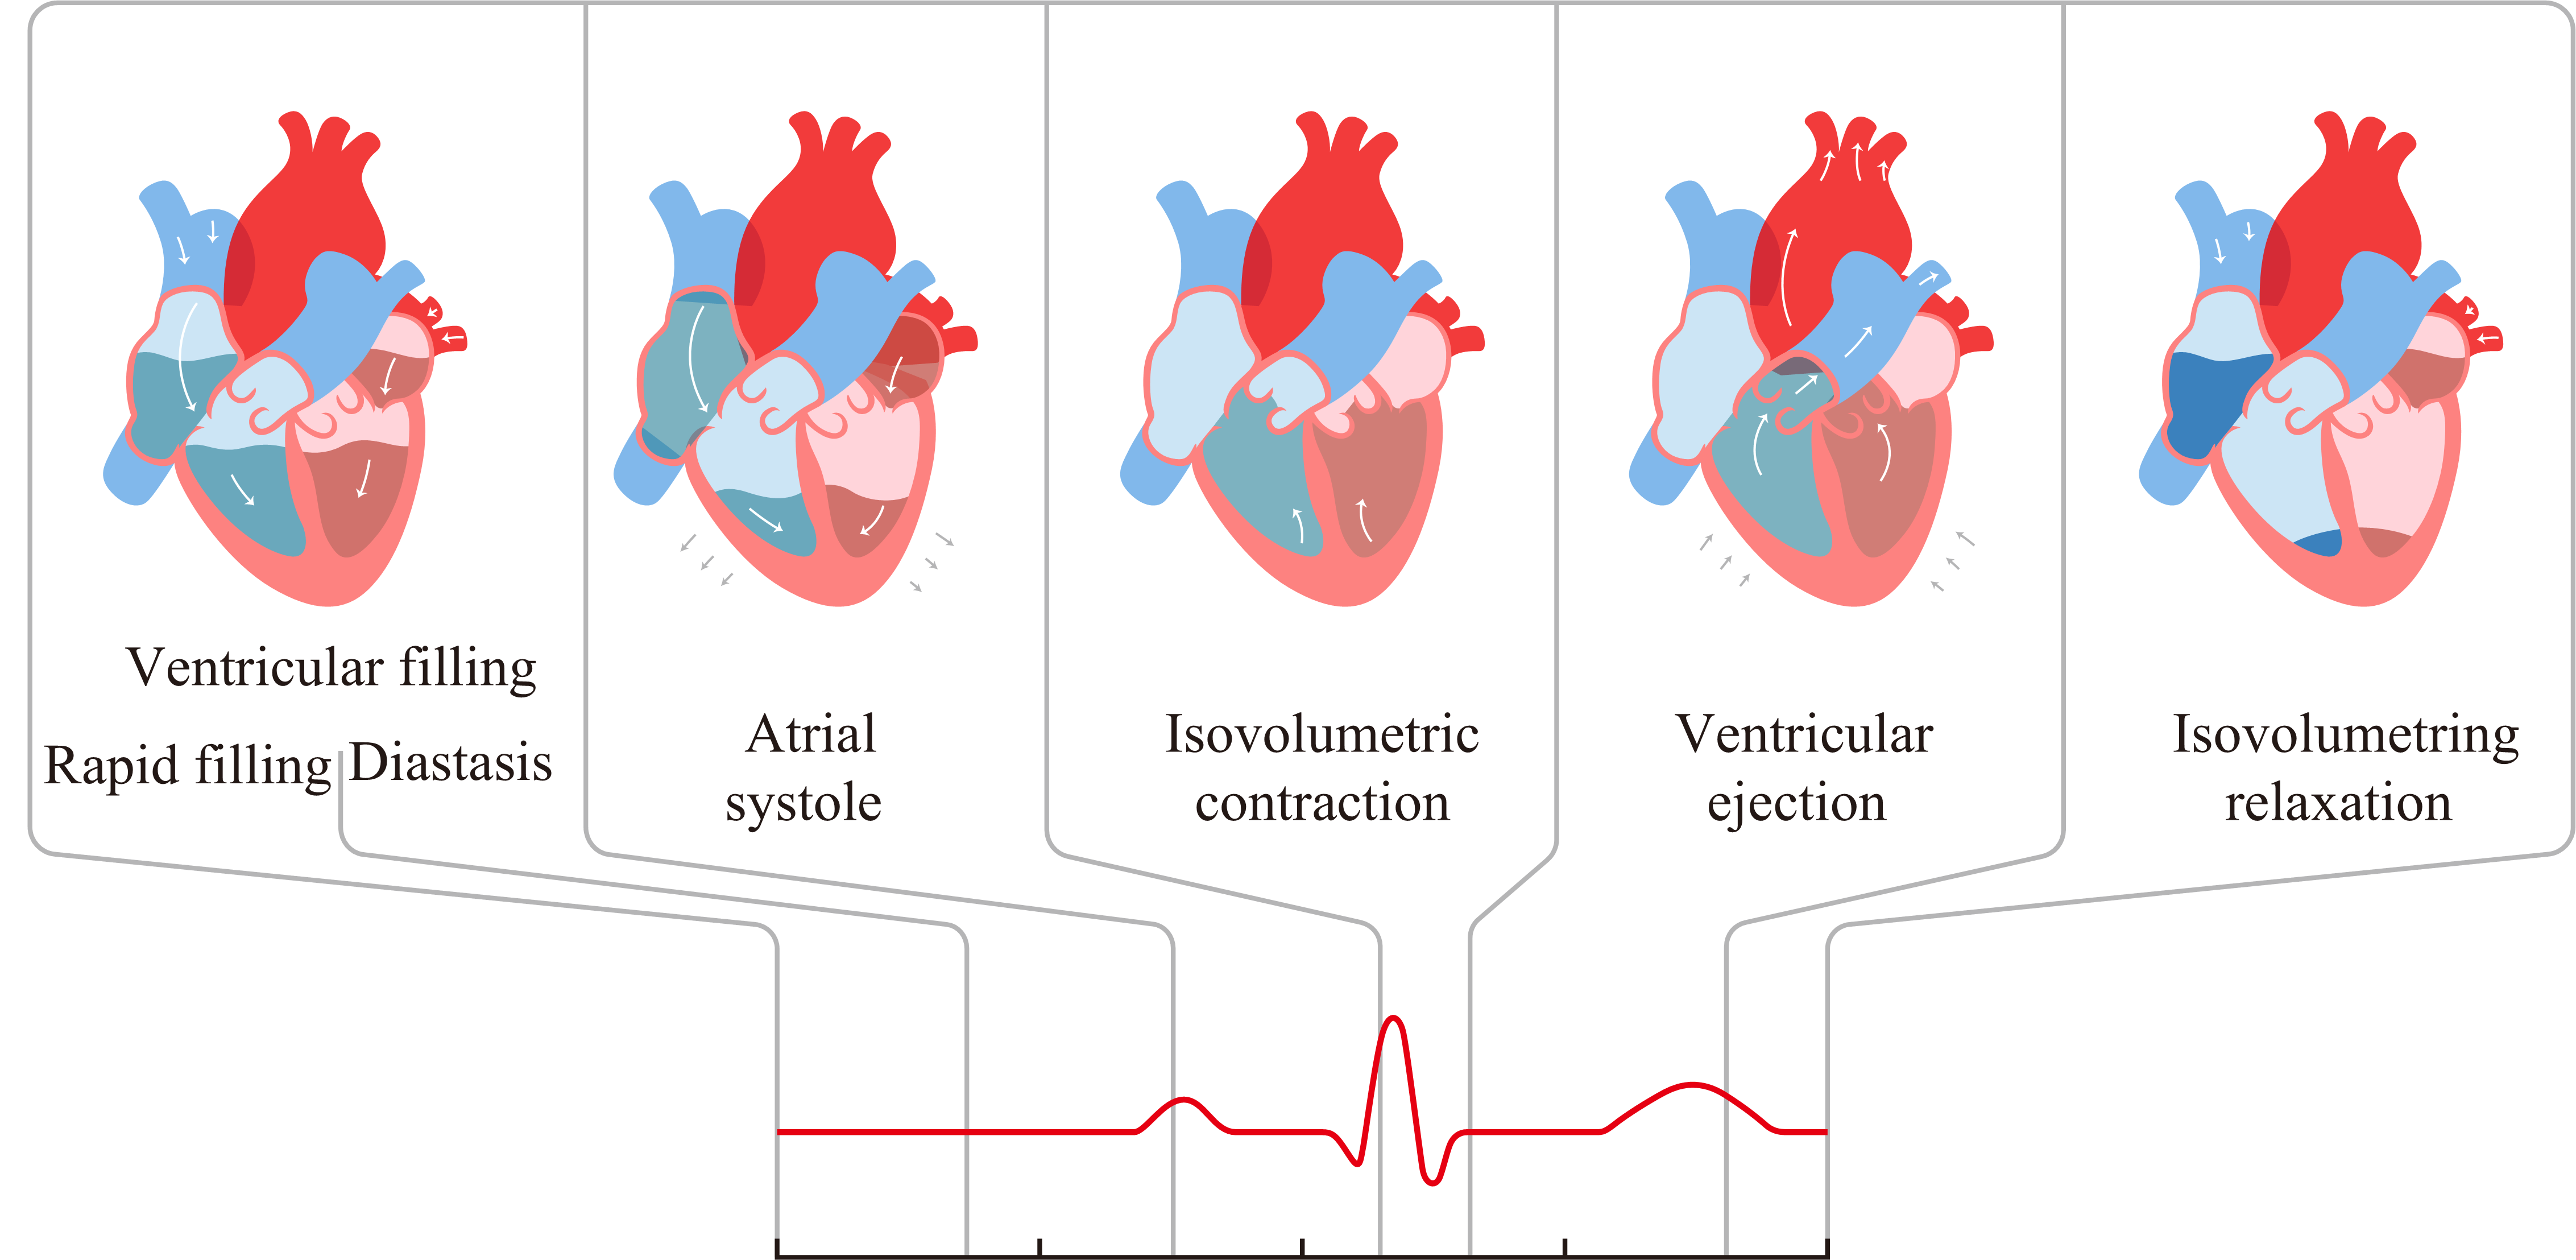
\includegraphics[width=8.5cm]{Figure/cycle}
    \caption{ Illustration of the cardiac cycle, correlating the key electrical events of the electrocardiogram (ECG) with their corresponding mechanical phases, such as atrial systole and ventricular ejection.}
    \label{fig:1}
\end{figure}

These foundational studies are indispensable first steps. However, a critical challenge emerges as research transitions from theoretical feasibility to clinical robustness. Many existing CIC transceiver designs, in their early stages, inevitably rely on static or averaged channel models~\cite{ryser2022modulation,bereuter2019leadless,khaleghi2020conductive}. This idealized approximation, while convenient for initial analysis, masks a crucial fact: the intracardiac channel dynamics exist on two distinct levels. The first level is the "healthy dynamic" ;
Fig.~\ref{fig:1} illustrates the regular heartbeat, which, even under normal sinus rhythm, induces predictable, periodic fluctuations in channel gain due to myocardial and hemodynamic shifts. However, the second, more severe level—and one that has been systematically overlooked—is the ``pathological dynamic." The channel environment induced by clinical conditions characterized by intermittent conduction failure is far from benign.

A representative form of such a condition, an Atrioventricular (AV) block, is shown in Fig.~\ref{fig:0}, is far from benign, exhibiting chaotic, drastic, and highly unpredictable fluctuations.


A representative form of such a condition, an Atrioventricular (AV) block, is shown in Fig.~\ref{fig:0}, which exhibits chaotic, drastic, and highly unpredictable fluctuations.


The vast majority of existing transceivers, lacking targeted consideration for these harsh "pathological dynamics," harbor a significant vulnerability when faced with real-world clinical challenges, forming a fundamental barrier to translating prototypes into clinically reliable devices.

The choice of receiver architecture becomes paramount in addressing this ultimate challenge. Given the extremely stringent constraints on power and complexity in LCPs, the Super-Regenerative Receiver (SRR) architecture emerges as one of the most promising candidates, by virtue of its inherent simplicity and immense potential for achieving high sensitivity at very low power~\cite{frey2013improved,macfarlane1948theory}. The SRR architecture, however, is a double-edged sword: its performance exhibits extreme sensitivity to variations in the input signal amplitude~\cite{chen2007fully,vidojkovic20112}. While this characteristic can be exploited for high gain under stable channel conditions, it transforms into a critical liability in the dynamic CIC environment we face, necessitating a sophisticated compensatory mechanism to unlock the SRR's full potential.

Therefore, Automatic Gain Control (AGC) is an indispensable component for ensuring system robustness.
Yet, conventional AGC solutions are not directly applicable to LCPs. Fully analog AGC systems, while offering rapid response, often suffer from poor linearity, imprecise gain control, and a fixed-threshold operation that limits adaptability in complex, varying environments~\cite{Zhao2023AnAF}.
Thus, fully digital AGC solutions, while capable of high precision and flexibility, come at the cost of significant computational overhead and power consumption, which is incompatible with the microwatt-level budget of an LCP~\cite{Li2020DigitalAC}.
Consequently, there is a pressing technological need for an AGC solution that optimally synergizes rapid response, precise control, and extreme power efficiency.

In response to this imperative, this paper introduces a novel SRR system integrated with a meticulously co-designed hybrid analog-digital AGC mechanism. This architecture strategically leverages the rapid response of an analog front-end  with the intelligent, fine-grained control afforded by digital processing, aiming to achieve robust compensation for dynamic CIC path gain variations while rigorously adhering to LCP power constraints. The main contributions of this work can be summarized as follows:

\begin{itemize}
    \item We propose a novel hybrid AGC receiver architecture, co-designed with an SRR, whose design principles can be extended to other IMDs operating in dynamic biological environments.
    \item We designed and implemented an \textit{ex-vivo} experimental platform capable of accurately emulating the dynamics of a representative pathological arrhythmia, providing a controllable and repeatable methodology for investigating communication challenges in harsh biological environments.

    \item For the first time, we systematically incorporate the complex channel dynamics induced by this representative clinical pathology into the entire design, optimization, and validation workflow of a transceiver, bridging a critical gap between existing research and clinical reality.

    \item This research provides valuable theoretical basis and a practical example for designing adaptive transceivers that can operate robustly in volatile biological environments, paving the way for the development of next-generation, high-performance, and high-reliability networked IMDs.
\end{itemize}

\begin{figure}[htbp]
    \centering
    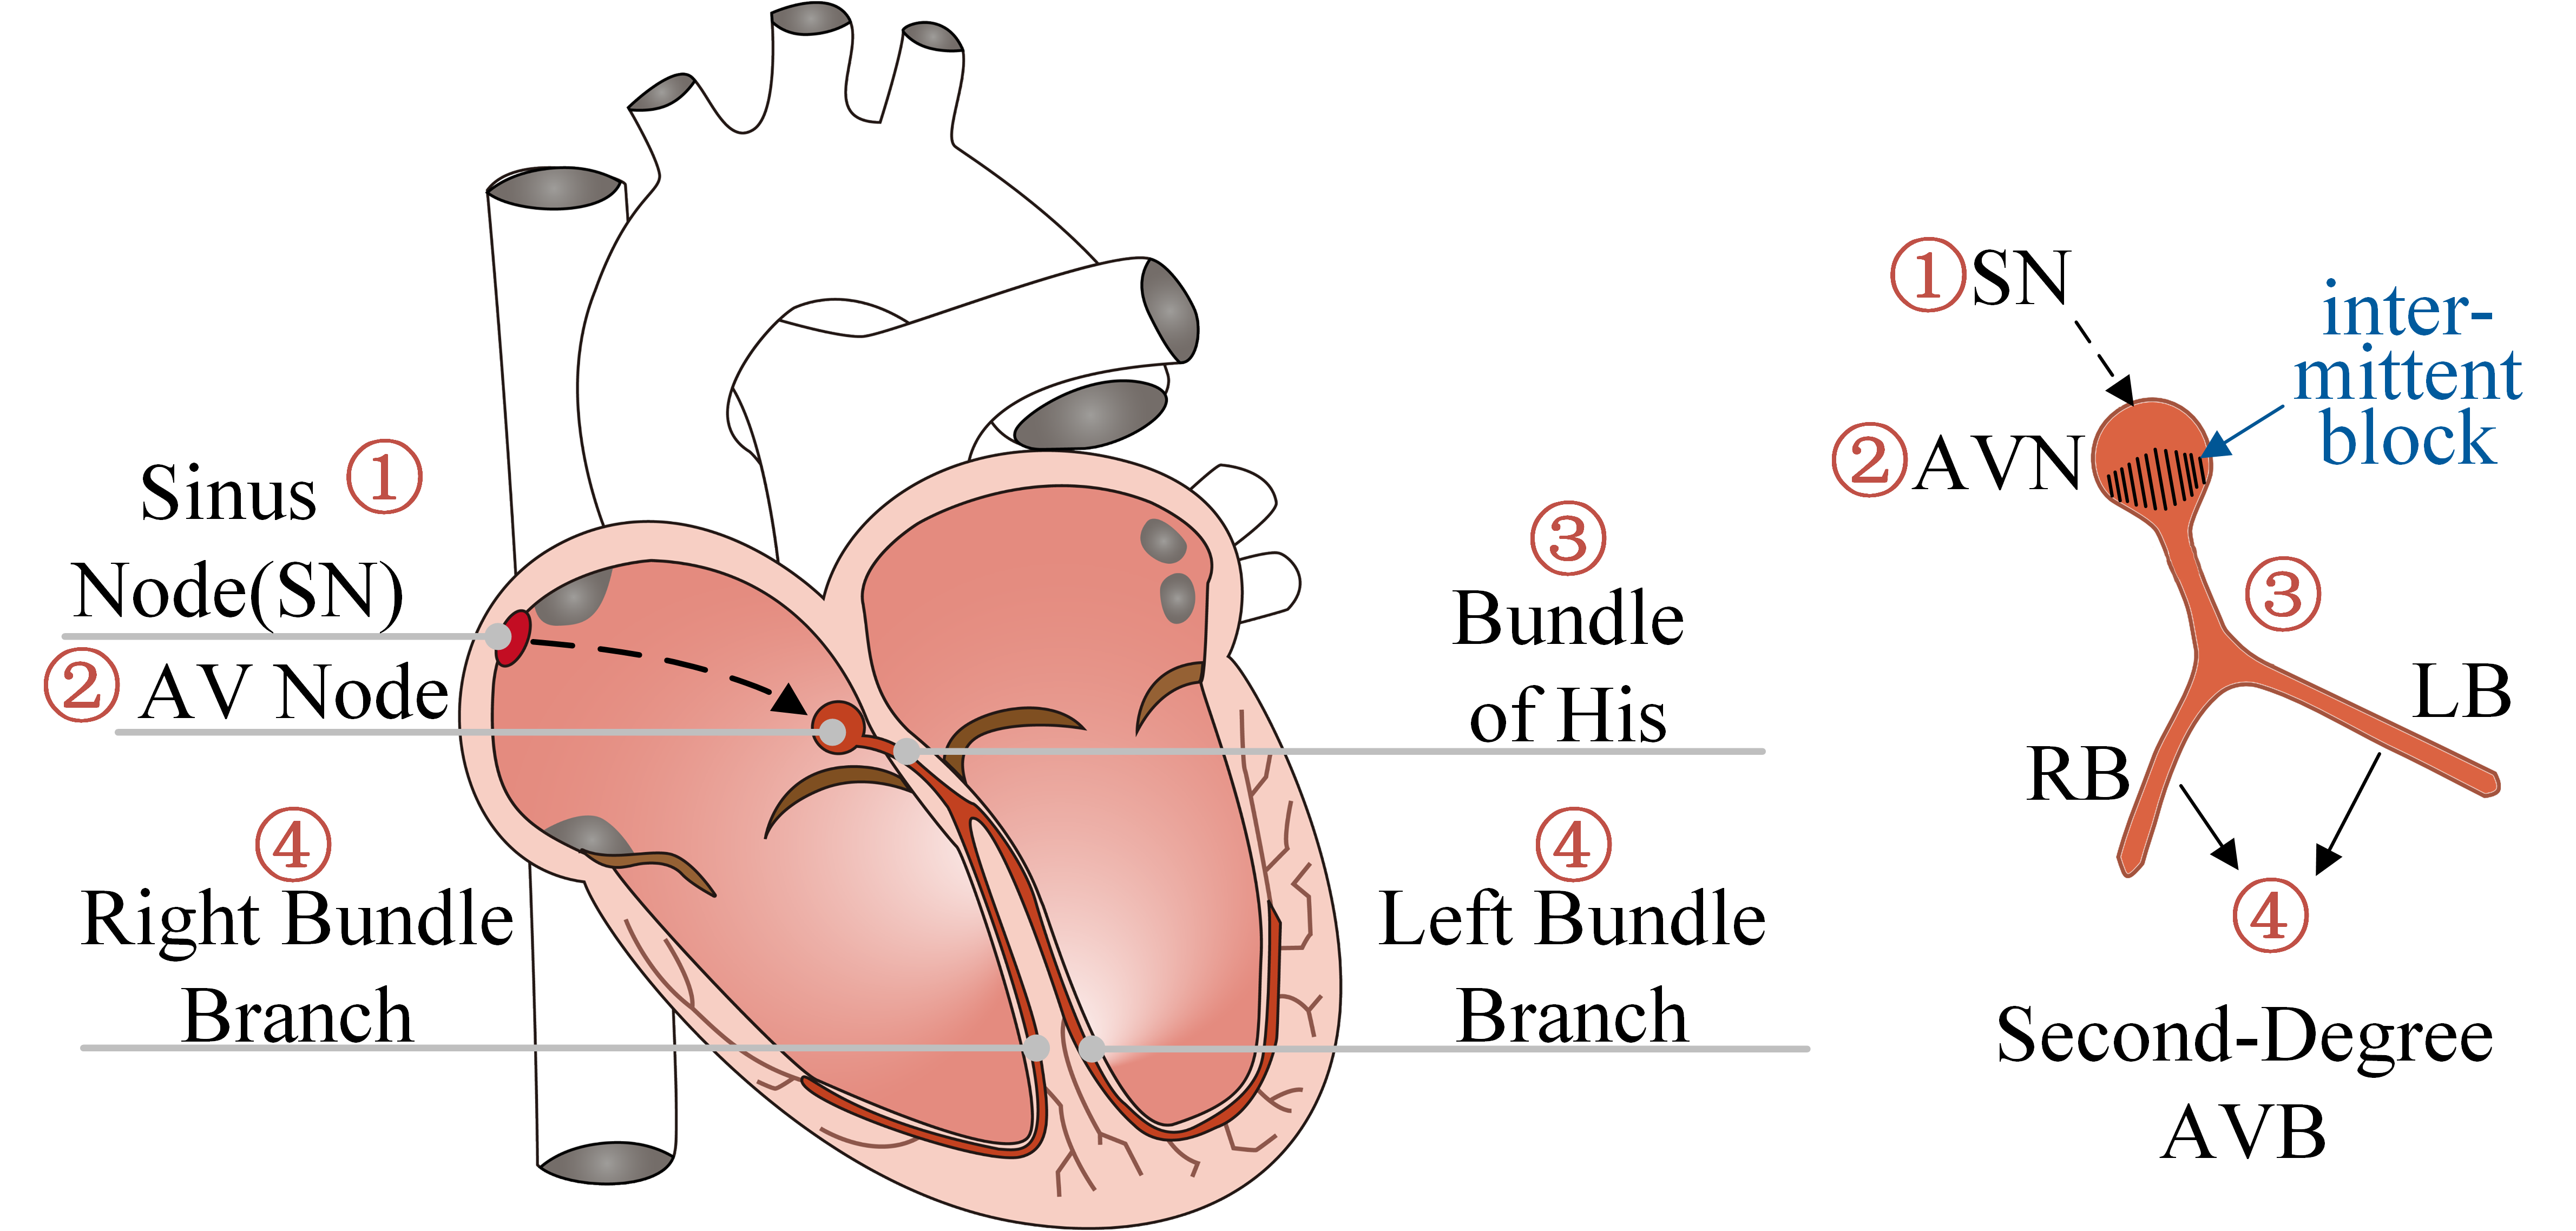
\includegraphics[width=8.3cm]{Figure/AVB}
    \caption{Schematic diagram of the cardiac conduction system and a representative Atrioventricular Block (Second-degree Type I).}
    \label{fig:0}
\end{figure}

\section{Methods}\label{sec:Methods}
\subsection{Dynamic Channel Characteristics and Impact on Receiver Performance}
\label{subsec:channel_and_impact}

Effective intra-cardiac communication (CIC) for multi-chamber leadless pacemakers is fundamentally constrained by the dynamic physiological environment. The rhythmic electromechanical activity of the heart induces profound temporal variations in the CIC channel gain, denoted as~$G_c(t)$~\cite{wei2024time}. This challenge is profoundly exacerbated under the very pathological conditions, such as arrhythmogenic profiles, that necessitate pacing. These conditions engender channel fluctuations that are far more complex, erratic, and severe than those observed during normal sinus rhythm. Maintaining reliable communication amidst such volatility constitutes a formidable and central challenge, which this work aims to address.

While the Super-Regenerative Receiver (SRR) architecture is an attractive candidate due to its high sensitivity and low power consumption, its performance is acutely dependent on the stability of its input signal amplitude,~$A_{in}(t)$. This sensitivity is an intrinsic consequence of its operating principle. A simplified equivalent parallel resonant circuit model of the SRR is shown in Fig.~\ref{fig:srr_model}.



\begin{figure}[h]
    \centering
    % Ensure this image file (srr_model.png) is in your LaTeX project directory.
    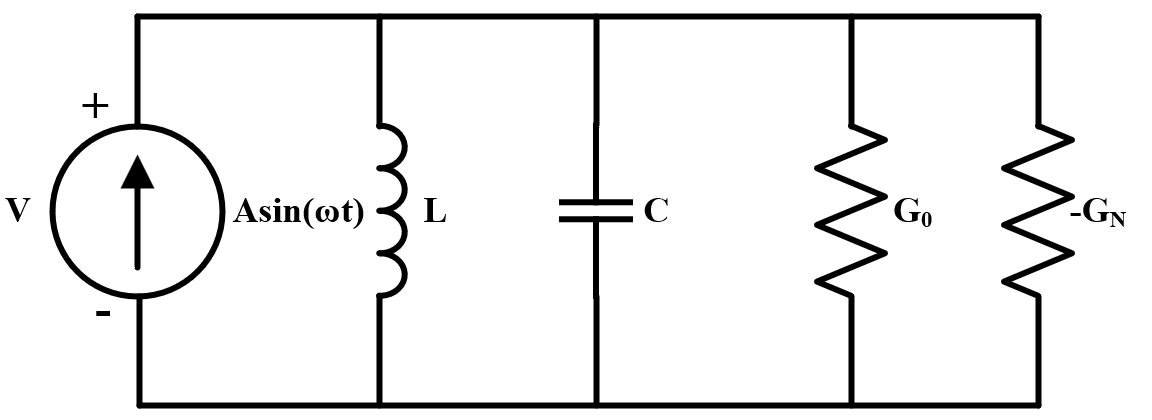
\includegraphics[width=0.7\columnwidth]{Figure/model}
    \caption{Equivalent parallel resonant circuit model of a super-regenerative oscillator, where the total conductance is~$G = G_o - G_N$.}
    \label{fig:srr_model}
\end{figure}

The core principle is predicated on periodically switching the oscillator's total parallel conductance,~$G$, between a negative value (the regeneration phase) and a positive value (the quenching phase). During regeneration, a negative conductance,~$-G_N$, provided by the active device, overcomes the tank's inherent losses,~$G_o$, yielding a net negative conductance~($G = G_o - G_N < 0$). This condition establishes an unstable positive feedback loop, wherein the tank voltage,~$V(t)$, grows exponentially from any initial perturbation. The voltage envelope,~$V_{env}(t)$, follows the relation:
\begin{equation}
    V_{env}(t) \propto e^{-\alpha t}, \quad \text{where} \quad \alpha = \frac{G}{2C}
    \label{eq:srr_growth}
\end{equation}
Since~$G < 0$, the damping factor~$\alpha$ is negative, resulting in exponential growth of the form~$e^{|\alpha|t}$. The input signal,~$A_{in}(t)$, serves as the initial "seed" for this exponential growth. Consequently, a stronger input signal yields a significantly larger final envelope amplitude over a fixed regeneration period.

In a front-end without adaptive control, the SRR's input amplitude,~$A_{in}(t)$, is directly modulated by the volatile channel gain:
\begin{equation}
    A_{in}(t) = G_{LNA} \cdot G_c(t) \cdot A_{tx}
    \label{eq:ain_channel}
\end{equation}
where~$G_{LNA}$~is the gain of the preceding Low Noise Amplifier and~$A_{tx}$~is the transmitted signal amplitude. As a direct consequence,~$A_{in}(t)$~experiences substantial variations synchronous with the cardiac cycle.

Since the SRR's output envelope is directly proportional to its input amplitude, $A_{in}(t)$, and signal power is proportional to the square of the amplitude, this input instability leads to a severe degradation in demodulation performance. The effective signal-to-noise ratio at the SRR's decision point, $SNR_{eff}(t)$, exhibits a quadratic dependence on the input signal amplitude:
\begin{equation}
    SNR_{eff}(t) = \kappa \frac{A_{in}(t)^2}{N_{eff}}
    \label{eq:snr_squared}
\end{equation}
where~$\kappa$~is a proportionality constant and~$N_{eff}$~is the equivalent input noise level. This quadratic relationship means that even moderate fluctuations in~$A_{in}(t)$~are magnified into severe variations in~$SNR_{eff}(t)$.

This cascade of dependencies results in a catastrophic decline in communication reliability. For On-Off Keying (OOK) modulation in an Additive White Gaussian Noise (AWGN) channel, the instantaneous bit error probability,~$P_e(t)$, is dictated by the complementary error function (erfc) of the instantaneous SNR:
\begin{equation}
    P_e(t) = \frac{1}{2}\text{erfc}\left(\sqrt{\frac{SNR_{eff}(t)}{2}}\right)
    \label{eq:Pe_t_revised}
\end{equation}

The overall, long-term Bit Error Rate (BER), being the time-averaged integral of~$P_e(t)$, has severe implications. During deep channel fades, the collapse of~$G_c(t)$~and consequently~$SNR_{eff}(t)$~causes~$P_e(t)$~to approach 0.5, signifying a momentary but complete link failure. Compounding this issue, the unstable input amplitude renders any fixed decision threshold,~$V_{th}$, inherently suboptimal, as the internal signal features leveraged for demodulation become highly variable. The confluence of these two critical issues---precipitous SNR degradation and the inherent suboptimality of a fixed decision threshold---provides the fundamental rationale and theoretical imperative for designing the adaptive compensation architecture that forms the basis of this work.

\subsection{Adaptive Receiver Architecture with Hybrid Gain Control}
\label{subsec:adaptive_architecture}
To counteract the severe performance degradation caused by dynamic channel fluctuations, we propose an adaptive receiver architecture incorporating a hybrid analog-digital Automatic Gain Control (AGC) loop. This approach is designed to stabilize the signal amplitude at the input of the Super-Regenerative Receiver (SRR) core, thereby ensuring robust demodulation under any channel condition. A schematic of this architecture, depicted in Fig.~\ref{fig:framework}, is a closed-loop feedback system engineered for the stringent power and complexity constraints of LCPs.


A key innovation of this architecture is its strategic exploitation of the self-quenching Super-Regenerative Receiver's (SRR) intrinsic operating principle.
The circuit schematic of the SRR core is shown in Fig. \ref{fig:sro_schematic}.


Unlike externally-quenched SRRs, our design employs an oscillator where the quenching mechanism is integrated directly into its own biasing network. This is achieved via a low-pass filter in the emitter path; as the oscillation envelope grows, rectified current charges this network, shifting the transistor's DC operating point to a non-oscillating region and thus intrinsically "quenching" the cycle.

The crucial aspect for amplification is that the incoming RF signal modulates this DC bias point. A stronger input signal creates a more favorable initial condition, which accelerates the oscillation build-up and produces a significantly larger output envelope within a single quenching period. This inherent characteristic—where the SRR's output envelope serves as a high-gain, amplified representation of its input amplitude—is precisely what our architecture leverages. It enables the SRR to function not only as a demodulator but also as a highly sensitive detector within the AGC feedback loop, forming a power-efficient solution for robust signal stabilization.


Leveraging the SRR's acute sensitivity to input amplitude, we have designed the following closed-loop feedback process to precisely stabilize this signal. The incoming RF signal from the CIC is first processed by a Low Noise Amplifier (LNA) to minimize noise figure degradation and is subsequently routed to a Variable Gain Amplifier (VGA), which serves as the primary gain control element. Its gain,~$G_{VGA}$, is dynamically modulated by an analog control voltage,~$V_c$.
After the VGA, a Received Signal Strength Indicator (RSSI) module measures the signal's amplitude and generates a proportional DC voltage.
This voltage is then digitized by an Analog-to-Digital Converter (ADC), yielding a discrete-time representation,~$A_{in,detected}(k)$, of the signal level for the microcontroller (MCU). The MCU executes a Proportional-Integral-Derivative (PID) control algorithm based on the discrepancy between this feedback value and a programmable setpoint to dynamically update the VGA's control voltage,~$V_c$. Concurrently, the main signal path proceeds from the VGA to the SRR core for demodulation. This architecture thus establishes a complete closed-loop control system, ensuring the amplitude of the signal presented to the SRR remains stable, irrespective of channel dynamics.


This hybrid architecture, with the SRR at the core of its feedback mechanism, strategically merges the distinct advantages of both the analog and digital domains. Its analog front-end (LNA, VGA) provides a rapid response to channel variations, while the digital back-end (MCU) enables the implementation of a precise, flexible, and robust control algorithm. In this synergistic configuration, the SRR functions not only as a demodulator but also as a highly efficient bridge connecting the analog gain stage to the digital controller. This architecture thereby overcomes the limitations of traditional fully-analog AGCs, which often suffer from suboptimal linearity and limited adaptability~\cite{Zhao2023AnAF}, while also avoiding the prohibitive power consumption and computational overhead that can be associated with fully-digital AGC schemes~\cite{Li2020DigitalAC}, thus offering a solution that balances performance and power consumption for implantable applications.



\begin{figure}[!t]
    \centering
    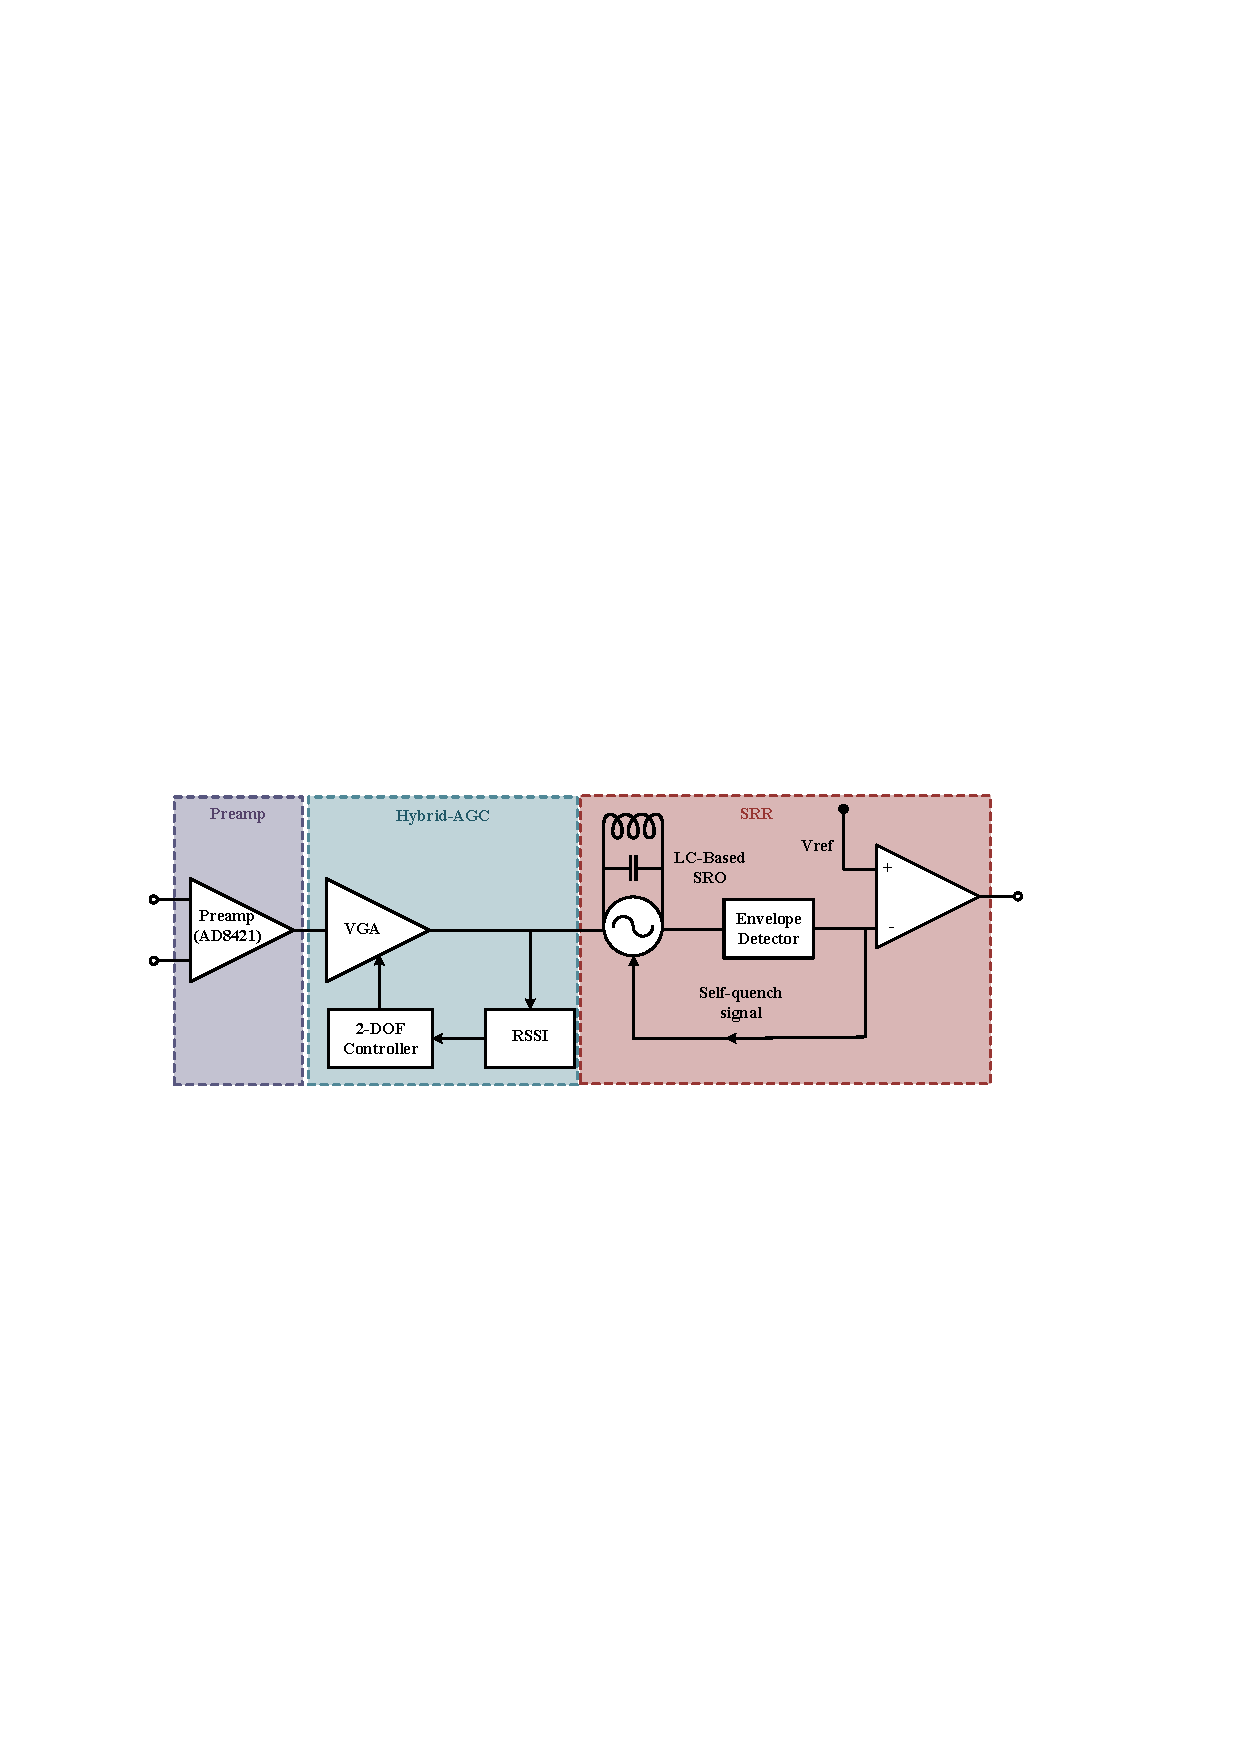
\includegraphics[width=8.3cm]{Figure/framework}
    \caption{Block diagram of the proposed adaptive receiver. The architecture comprises three main sections: a Preamplifier (Preamp), a Hybrid-AGC loop to stabilize the signal level, and a Super-Regenerative Receiver (SRR) core for demodulation. The SRR employs a self-quenching oscillator (SRO) for power-efficient operation.}
    \label{fig:framework}
\end{figure}






\subsection{Gain Compensation Principle and PID Control Algorithm}
\label{subsec:principle_and_algorithm}

The fundamental principle of the proposed AGC system is to dynamically adjust the VGA gain, $G_{VGA}$, to counteract the channel gain variations, $G_c(t)$, thereby maintaining a constant signal amplitude, $V_{target}$, at the SRR input. When the AGC loop achieves a stable or quasi-stable state, the relationship between the required $G_{VGA}$ and the instantaneous $G_c(t)$ can be derived from the overall system gain expression $A_{in,AGC}(t) = G_{VGA}(V_c,t) \cdot G_{LNA} \cdot G_c(t) \cdot A_{tx}$. By setting $A_{in,AGC}(t) \approx V_{target}$, the requisite VGA gain is:
\begin{equation}
    G_{VGA}(t) \approx \frac{V_{target}}{G_{LNA} \cdot G_c(t) \cdot A_{tx}}
    \label{eq:GVGA_compensation}
\end{equation}


Equation~\eqref{eq:GVGA_compensation} lucidly illustrates that the AGC system must modulate $G_{VGA}(t)$ to be approximately inversely proportional to the instantaneous channel gain. This self-regulating action is orchestrated by a Proportional-Integral-Derivative (PID) controller implemented in the digital domain. For robust and efficient implementation, an incremental PID formulation is employed~\cite{wang2022incremental}, where the controller calculates the necessary control effort increment, $\Delta u_k$, at each time step. This is derived from the standard discrete-time representation of a PID controller:


\begin{equation}
    \Delta u_k = K_p (e_k - e_{k-1}) + K_i T_s e_k + \frac{K_d}{T_s} (e_k - 2e_{k-1} + e_{k-2})
    \label{eq:PID_standard_discrete}
\end{equation}
where $K_p, K_i, K_d$ are the proportional, integral, and derivative gains, and $T_s$ is the sampling period. For efficient implementation, this equation is rearranged by grouping terms based on the error samples:
\begin{equation}
    \Delta u_k = (K_p + K_i T_s + \frac{K_d}{T_s}) e_k - (K_p + \frac{2K_d}{T_s}) e_{k-1} + (\frac{K_d}{T_s}) e_{k-2}
    \label{eq:PID_rearranged}
\end{equation}
This can be expressed in a more direct computational form:
\begin{equation}
    \Delta u_k = k_1 e_k - k_2 e_{k-1} + k_3 e_{k-2}
    \label{eq:PID_computational_form}
\end{equation}
where the coefficients $k_1 = K_p + K_i T_s + K_d/T_s$, $k_2 = K_p + 2K_d/T_s$, and $k_3 = K_d/T_s$ are pre-calculated to optimize the real-time control loop. The cumulative digital control output, $u_k = u_{k-1} + \Delta u_k$, is then converted by the DAC. The detailed iterative process is presented in Algorithm~\ref{alg:pid_control}.The selection of the PID controller gains ($K_p$, $K_i$, and $K_d$) was performed through a systematic, empirical tuning process directly on the experimental platform. The tuning procedure was as follows: Initially, $K_i$ and $K_d$ were set to zero, and the proportional gain ($K_p$) was gradually increased until the system exhibited a sufficiently fast response to a step change in the channel. Subsequently, the integral gain ($K_i$) was introduced to eliminate the residual steady-state error, ensuring the output signal could precisely stabilize around the target level. Finally, the derivative gain ($K_d$) was carefully adjusted to dampen the overshoot and oscillations introduced by $K_p$ and $K_i$, thereby improving the dynamic tracking performance during the sharp and rapid channel fluctuations characteristic of the emulated Atrioventricular Block (AVB). The final set of parameters demonstrated good stability and compensation performance across all tested heart preparations.


The choice of a PID controller, as opposed to simpler control schemes like PI or P-only, is a deliberate design decision to handle the complex dynamics of the CIC. A simple P-controller would suffer from steady-state error, failing to lock the signal precisely to $V\_target$. While a PI controller could eliminate this error, it would struggle to react to the sharp, unpredictable channel changes characteristic of a `dropped beat' in an AVB cycle. The derivative (D) term is therefore crucial; it provides an anticipatory response to rapid changes in the channel gain, minimizing transient errors during these abrupt hemodynamic shifts. This sophisticated control is paramount for ensuring dependable communication under the most challenging physiological conditions.




\begin{figure}[!t]
    \centering
    % 确保你的图片文件名和路径正确
    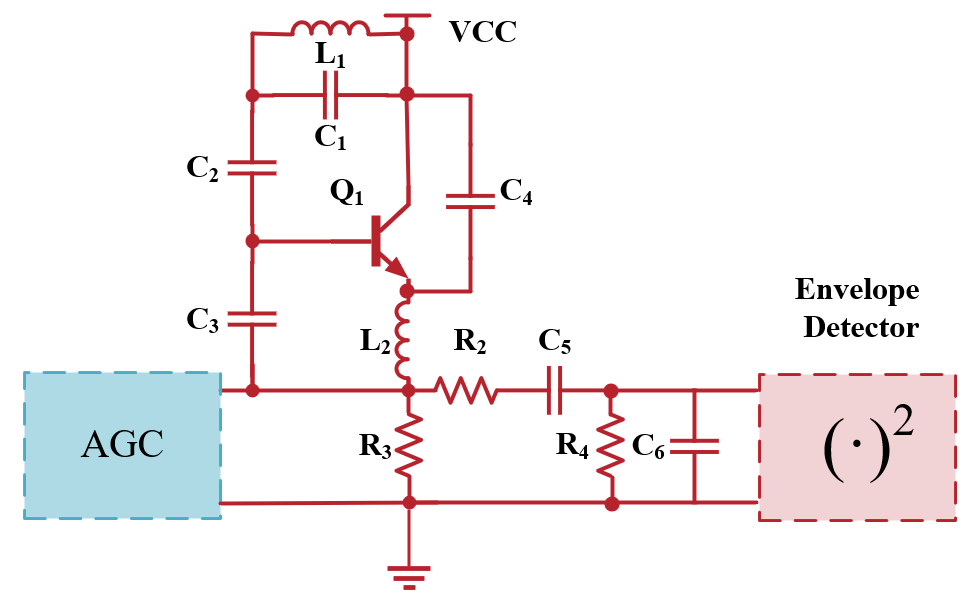
\includegraphics[width=0.75\columnwidth]{Figure/SRO}
    \caption{Circuit schematic of the self-quenching oscillator core. The self-quenching action is intrinsically governed by the transistor's biasing network.}
    \label{fig:sro_schematic} % 给它一个清晰的标签
\end{figure}





\begin{algorithm}[H]
    \caption{SRR Input Stabilization Algorithm}
    \label{alg:pid_control}
    \begin{algorithmic}[1] % The [1] enables line numbering
        \Require
            $V_{\text{target,dig}}$, $k_1, k_2, k_3$, $u_{\text{min\_dig}}, u_{\text{max\_dig}}$
        \Ensure
            $V_c(k)$

        \State Initialize $u_{\text{prev}}$; $e_{\text{prev1}} \gets 0$; $e_{\text{prev2}} \gets 0$
        \While{system is operating}
            \State $A_{\text{in,detected}}(k) \gets \text{Sample And Digitize SRR Input}()$
            \State $e_k \gets V_{\text{target,dig}} - A_{\text{in,detected}}(k)$
            \State $\Delta u_k \gets k_1 e_k - k_2 e_{\text{prev1}} + k_3 e_{\text{prev2}}$
            \State $u_k \gets u_{\text{prev}} + \Delta u_k$
            \State $u_k \gets \text{saturate}(u_k, u_{\text{min\_dig}}, u_{\text{max\_dig}})$

%            \Comment{Apply output limits}
            \State $V_c(k) \gets \text{Digital To Analog Conversion}(u_k)$
            \State $\text{Set VGA Control Voltage}(V_c(k))$
            \State \hspace{-1.5em} $\triangleright$ Update historical values for next iteration %
            \State $e_{\text{prev2}} \gets e_{\text{prev1}}$
            \State $e_{\text{prev1}} \gets e_k$
            \State $u_{\text{prev}} \gets u_k$
        \EndWhile
    \end{algorithmic}
\end{algorithm}




\section{Experimental Methodology and Setup}

The efficacy of the proposed AGC system was rigorously validated through a comprehensive \textit{ex-vivo} experimental methodology. This methodology encompassed the quantitative characterization of dynamic intracardiac channels and the subsequent end-to-end performance evaluation of the adaptive receiver operating within this emulated environment.

\subsection{Dynamic Channel Emulation Platform and Characterization}

The cornerstone of the experimental methodology was an \textit{ex-vivo} perfusion platform, initially configured for fundamental channel characterization as depicted in Fig.~\ref{fig:agc_test_schematic}.
The biological core of the platform comprised a fresh porcine heart, procured from a local abattoir and selected based on criteria ensuring structural and physiological similarity to human hearts, including a weight range of 90 to 120 kg and considerations for cell turnover rate~\cite{karacolak2012dielectric}. Hemodynamic emulation was achieved via a dual-channel peristaltic pump system, which circulated a perfusate through the cardiac chambers. The perfusate was a physiologically relevant simulated blood, formulated with deionized water and sodium chloride to precisely match the electrical conductivity of native human blood at 37°C.
This formulation adhered to established methodologies~\cite{maldari2020wide, gabriel1996dielectric}, and its conductivity profile was verified against real blood across the operational frequency spectrum from 100~kHz to 20~MHz. The governing relationship for the conductivity of the NaCl solution is given by~\cite{gadani2012effect}.





\begin{figure}[!t]
    \centering
    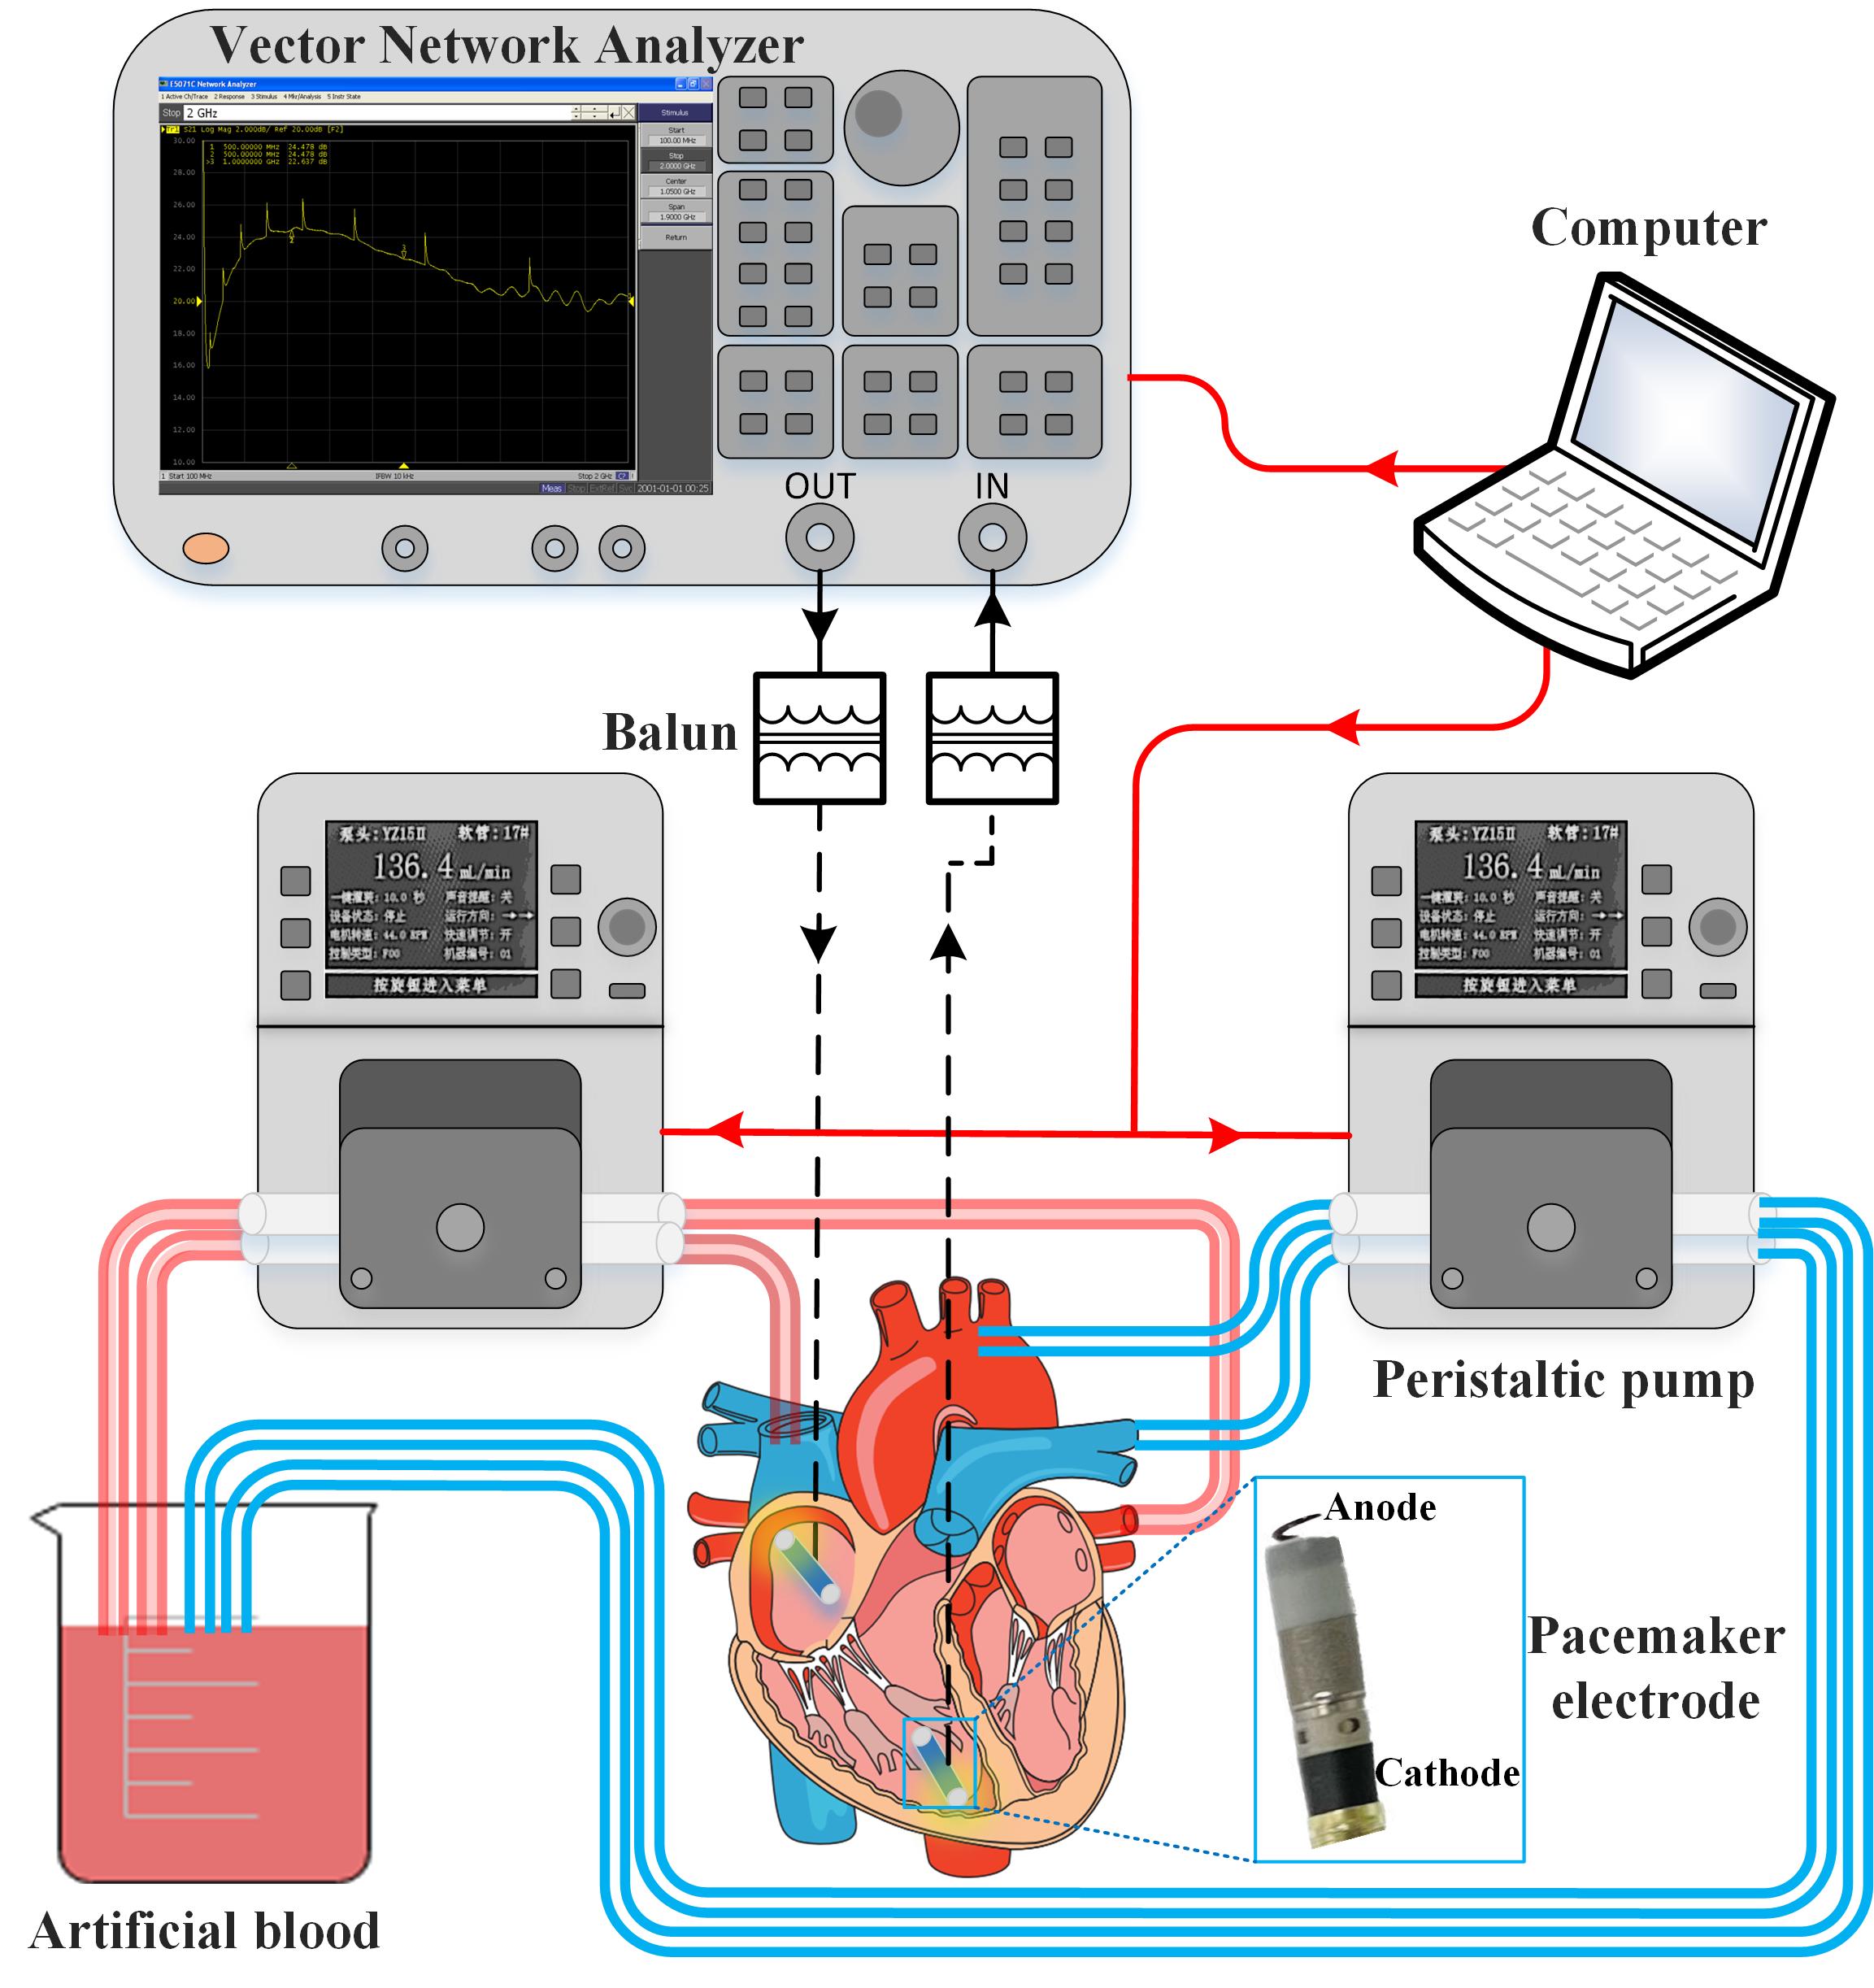
\includegraphics[width=0.9\columnwidth]{Figure/measure_setup.png}
    \caption{Photograph of the assembled experimental testbed, showcasing the peristaltic pump system, the cannulated \textit{ex-vivo} porcine heart, the signal generation instrumentation, and the custom-developed receiver module.1:1 baluns are used at the transmitter and receiver interfaces for galvanic isolation.}
    \label{fig:agc_test_schematic}
\end{figure}

\begin{table}[!t] % 如果您有这个表格，可以保留并重命名label
\centering
\caption{Cardiac Cycle Phases and Corresponding Chamber Volumes Utilized for Dynamic Simulation}
\begin{tabular}{cccc}
\hline
\text{\bfseries Phase} & \text{\bfseries Duration(s)} & \text{\begin{tabular}[c]{@{}c@{}}\bfseries Left Cardiac\\\bfseries Volume (mL)\end{tabular}} & \text{\begin{tabular}[c]{@{}c@{}}\bfseries Right Cardiac\\ \bfseries Volume (mL)\end{tabular}} \\ \hline
\text{\begin{tabular}[c]{@{}c@{}}\bfseries Isovolumetric\\ \bfseries Relaxation\end{tabular}} & 0.07 & 120.00 & 150.00 \\
\text{\bfseries Rapid filling} & 0.11 & 173.44 & 202.88 \\
\text{\bfseries Diastasis} & 0.22 & 191.25 & 220.50 \\
\text{\begin{tabular}[c]{@{}c@{}}\bfseries Atrial\\\bfseries  Contraction\end{tabular}} & 0.10 & 215.00 & 244.00 \\
\text{\begin{tabular}[c]{@{}c@{}}\bfseries Isovolumetric\\\bfseries  Contraction\end{tabular}} & 0.05 & 215.00 & 244.00 \\
\text{\bfseries Rapid ejection} & 0.10 & 151.67 & 181.34 \\
\text{\bfseries Slow ejection} & 0.15 & 120.00 & 150.00 \\ \hline
\end{tabular}
\label{tab:volume_data}
\end{table}


A host computer served as the central controller, communicating with the pumps (Model: BL400H/2*YZ15III) via an RS-232 serial interface. Through a network of silicone tubing securely cannulated to the heart's major vessels, the system precisely governed the flow of the simulated blood.
Custom-developed serial control software (SSCOM V5.13) enabled the dynamic adjustment of pump speed and direction, granting us the capability for meticulous, time-varying control over intracardiac chamber volumes.

To validate our system under challenging pathological dynamics, we selected Atrioventricular Block (AVB)—a condition characterized by intermittent conduction failure—as our model arrhythmia. Among the different types of AVB, Mobitz Type I presents an ideal and comprehensive test case for an adaptive system, as its characteristic Wenckebach phenomenon includes both progressive changes and an eventual abrupt ``dropped beat." An adaptive system that can successfully track this complex pattern demonstrates its capability to handle both gradual and sudden channel variations. Therefore, our platform was programmed to precisely replicate the hemodynamic profile of the AVB, serving as a representative model for a harsh pathological channel environment.

These profiles, with quantitative data detailed in TABLE~\ref{tab:volume_data}, were carefully designed based on comprehensive analyses of published human cardiac chamber volume data and motion patterns~\cite{maceira2010reference, 2006Normalized, 2006Reference, 2013Reference, chen2022investigation}.
The resulting dynamic mappings are illustrated in Fig.~\ref{fig:nsr_mapping} and Fig.~\ref{fig:avb_mapping}. The emulation was meticulously programmed by first discretizing the target volumetric curve for each condition into its constituent cardiac phases. For each phase, the necessary average flow rate was calculated. The host computer then executed a pre-programmed sequence of serial commands to precisely control the pumps' flow rates and durations for each segment. For instance, to accurately simulate the ``dropped beat'' characteristic of our AVB model, the control sequence included a programmed atrial filling period that was not followed by a corresponding ventricular ejection. This ability to recreate distinct, non-uniform channel behaviors was critical for both channel characterization and receiver evaluation. For initial characterization, a Vector Network Analyzer (VNA) was integrated with the platform to continuously measure the RA-RV channel's path gain.


\begin{figure}[!t]
    \centering
    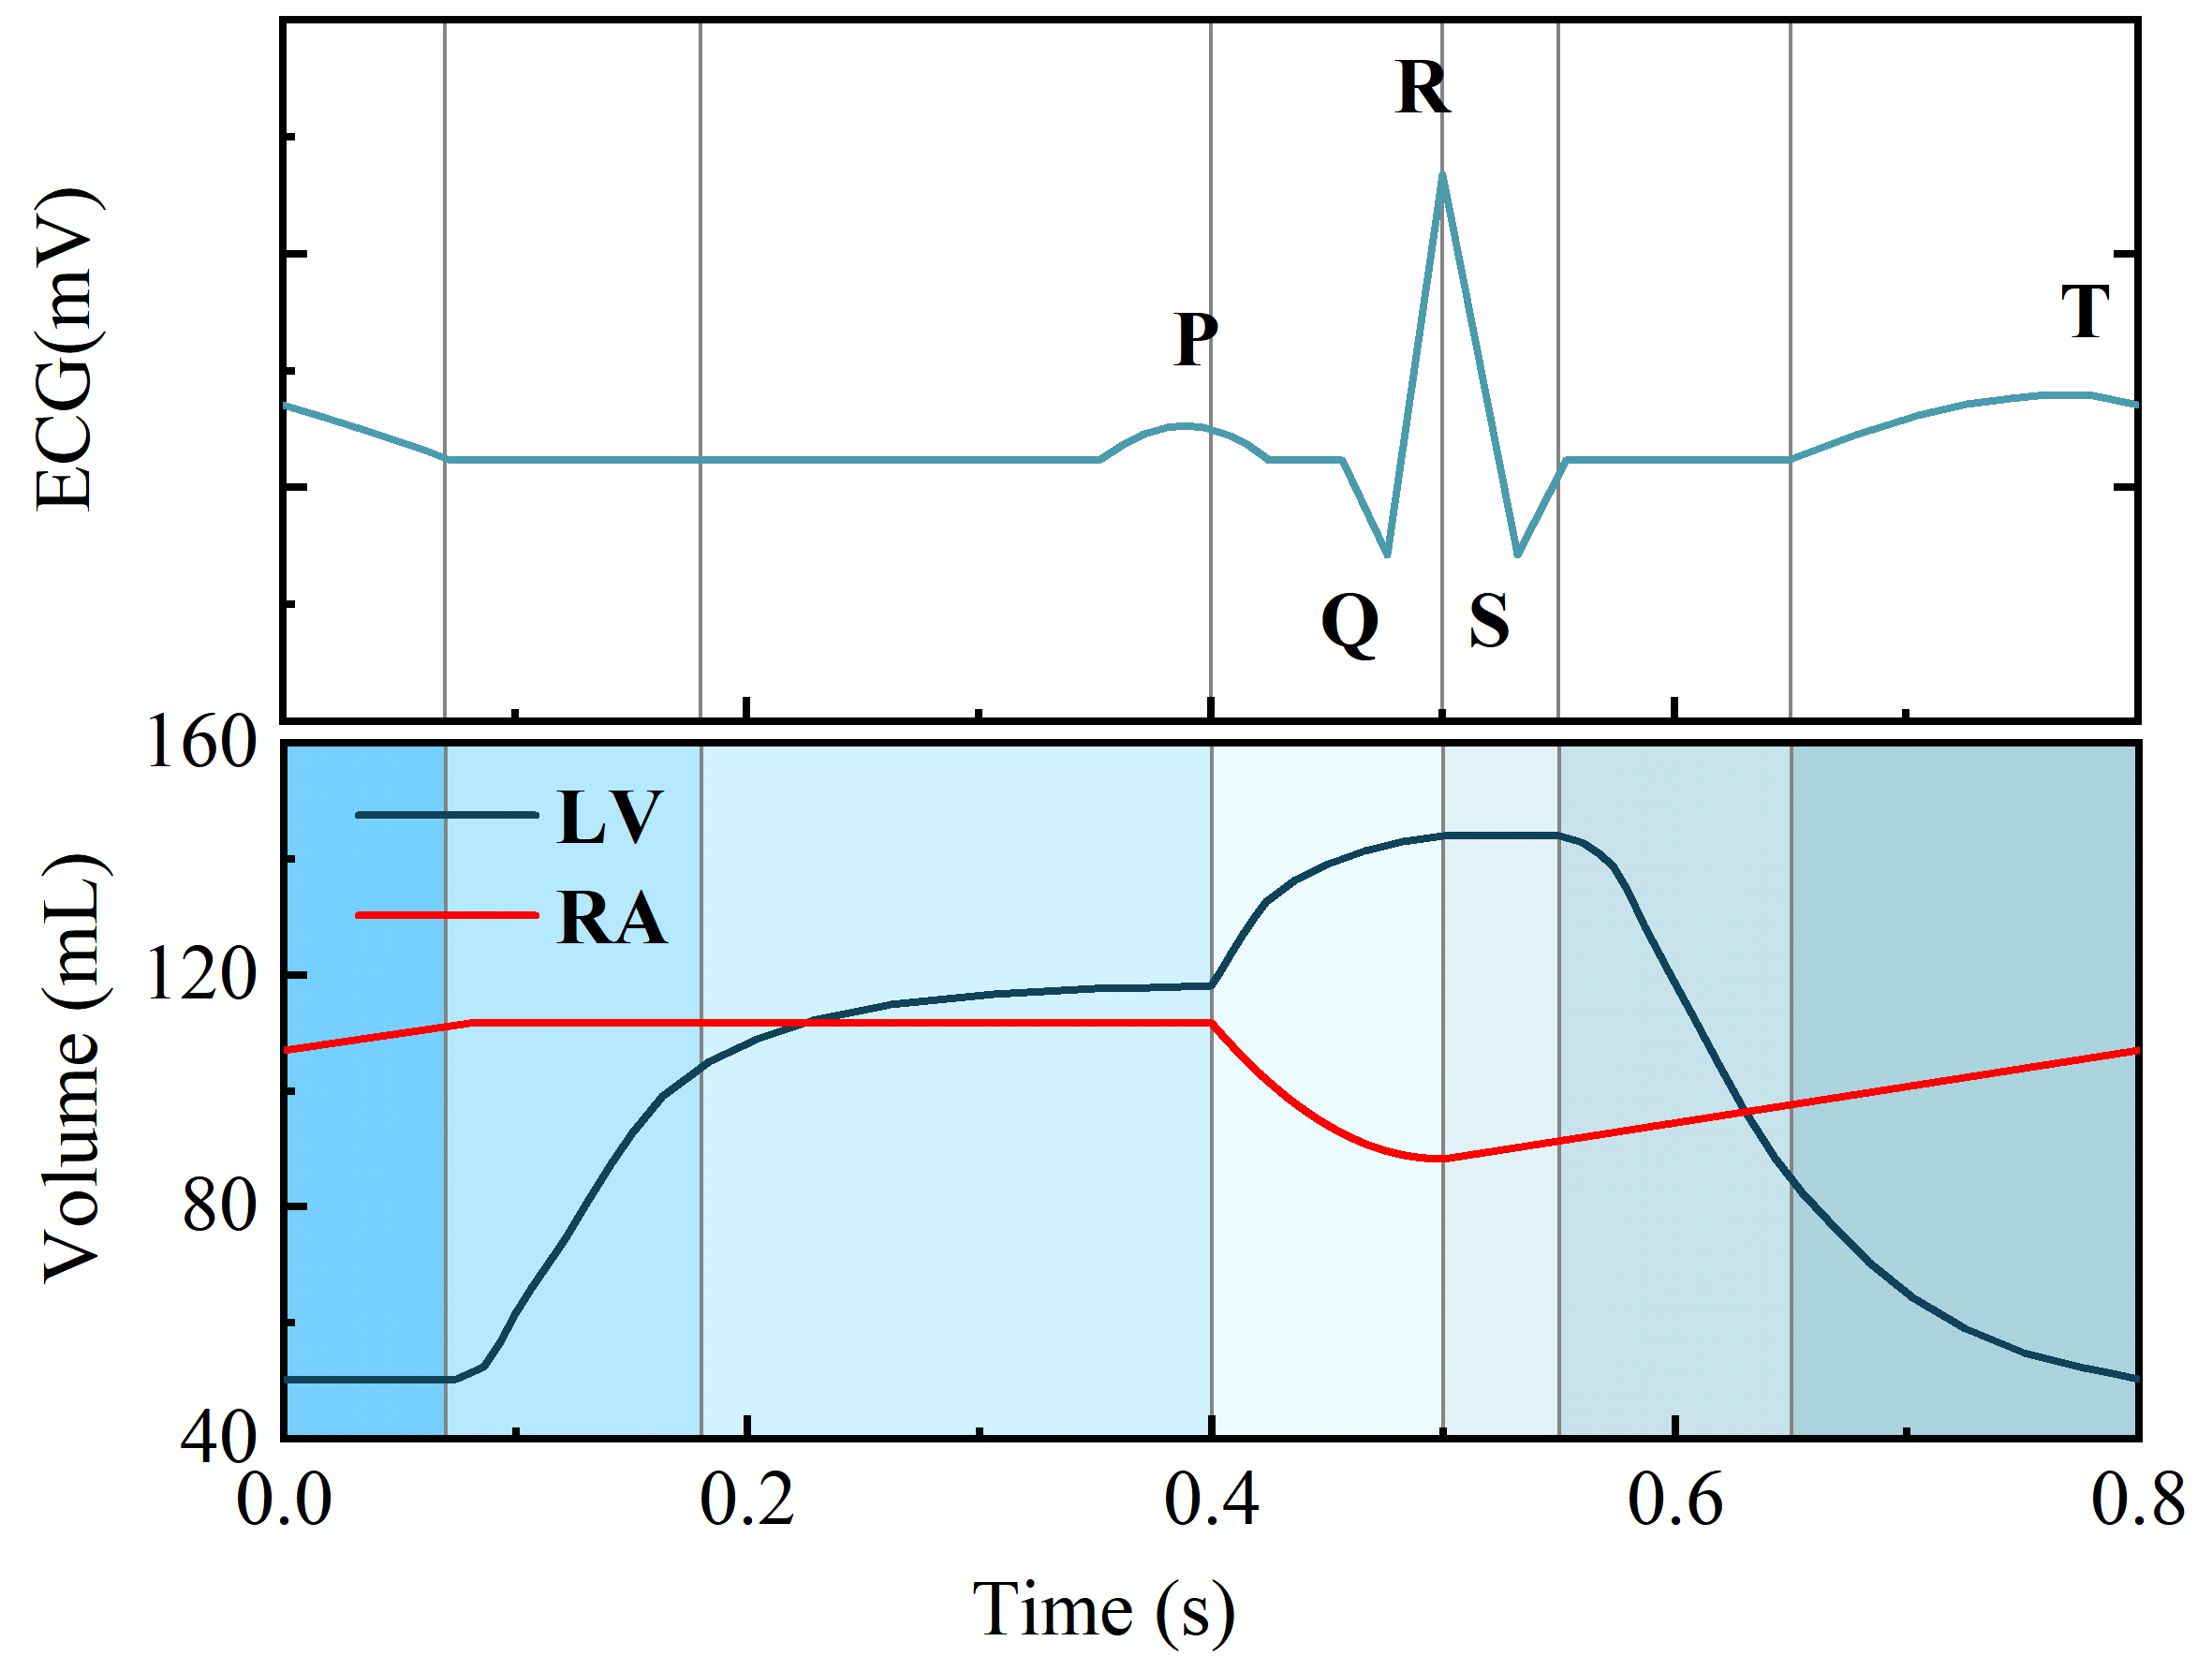
\includegraphics[width=0.9\columnwidth]{Figure/Nor_Vol} % 使用您的第三张图 (IMG_4224.jpeg)
    \caption{Dynamic mapping relationship between the electrocardiogram (ECG) and right-sided chamber volumes (RA and RV) under simulated Normal Sinus Rhythm (NSR). This volumetric profile served as the baseline model for a healthy heart and formed the basis for emulating pathological conditions.
.}
    \label{fig:nsr_mapping}
\end{figure}


\begin{figure}[!t]
    \centering
    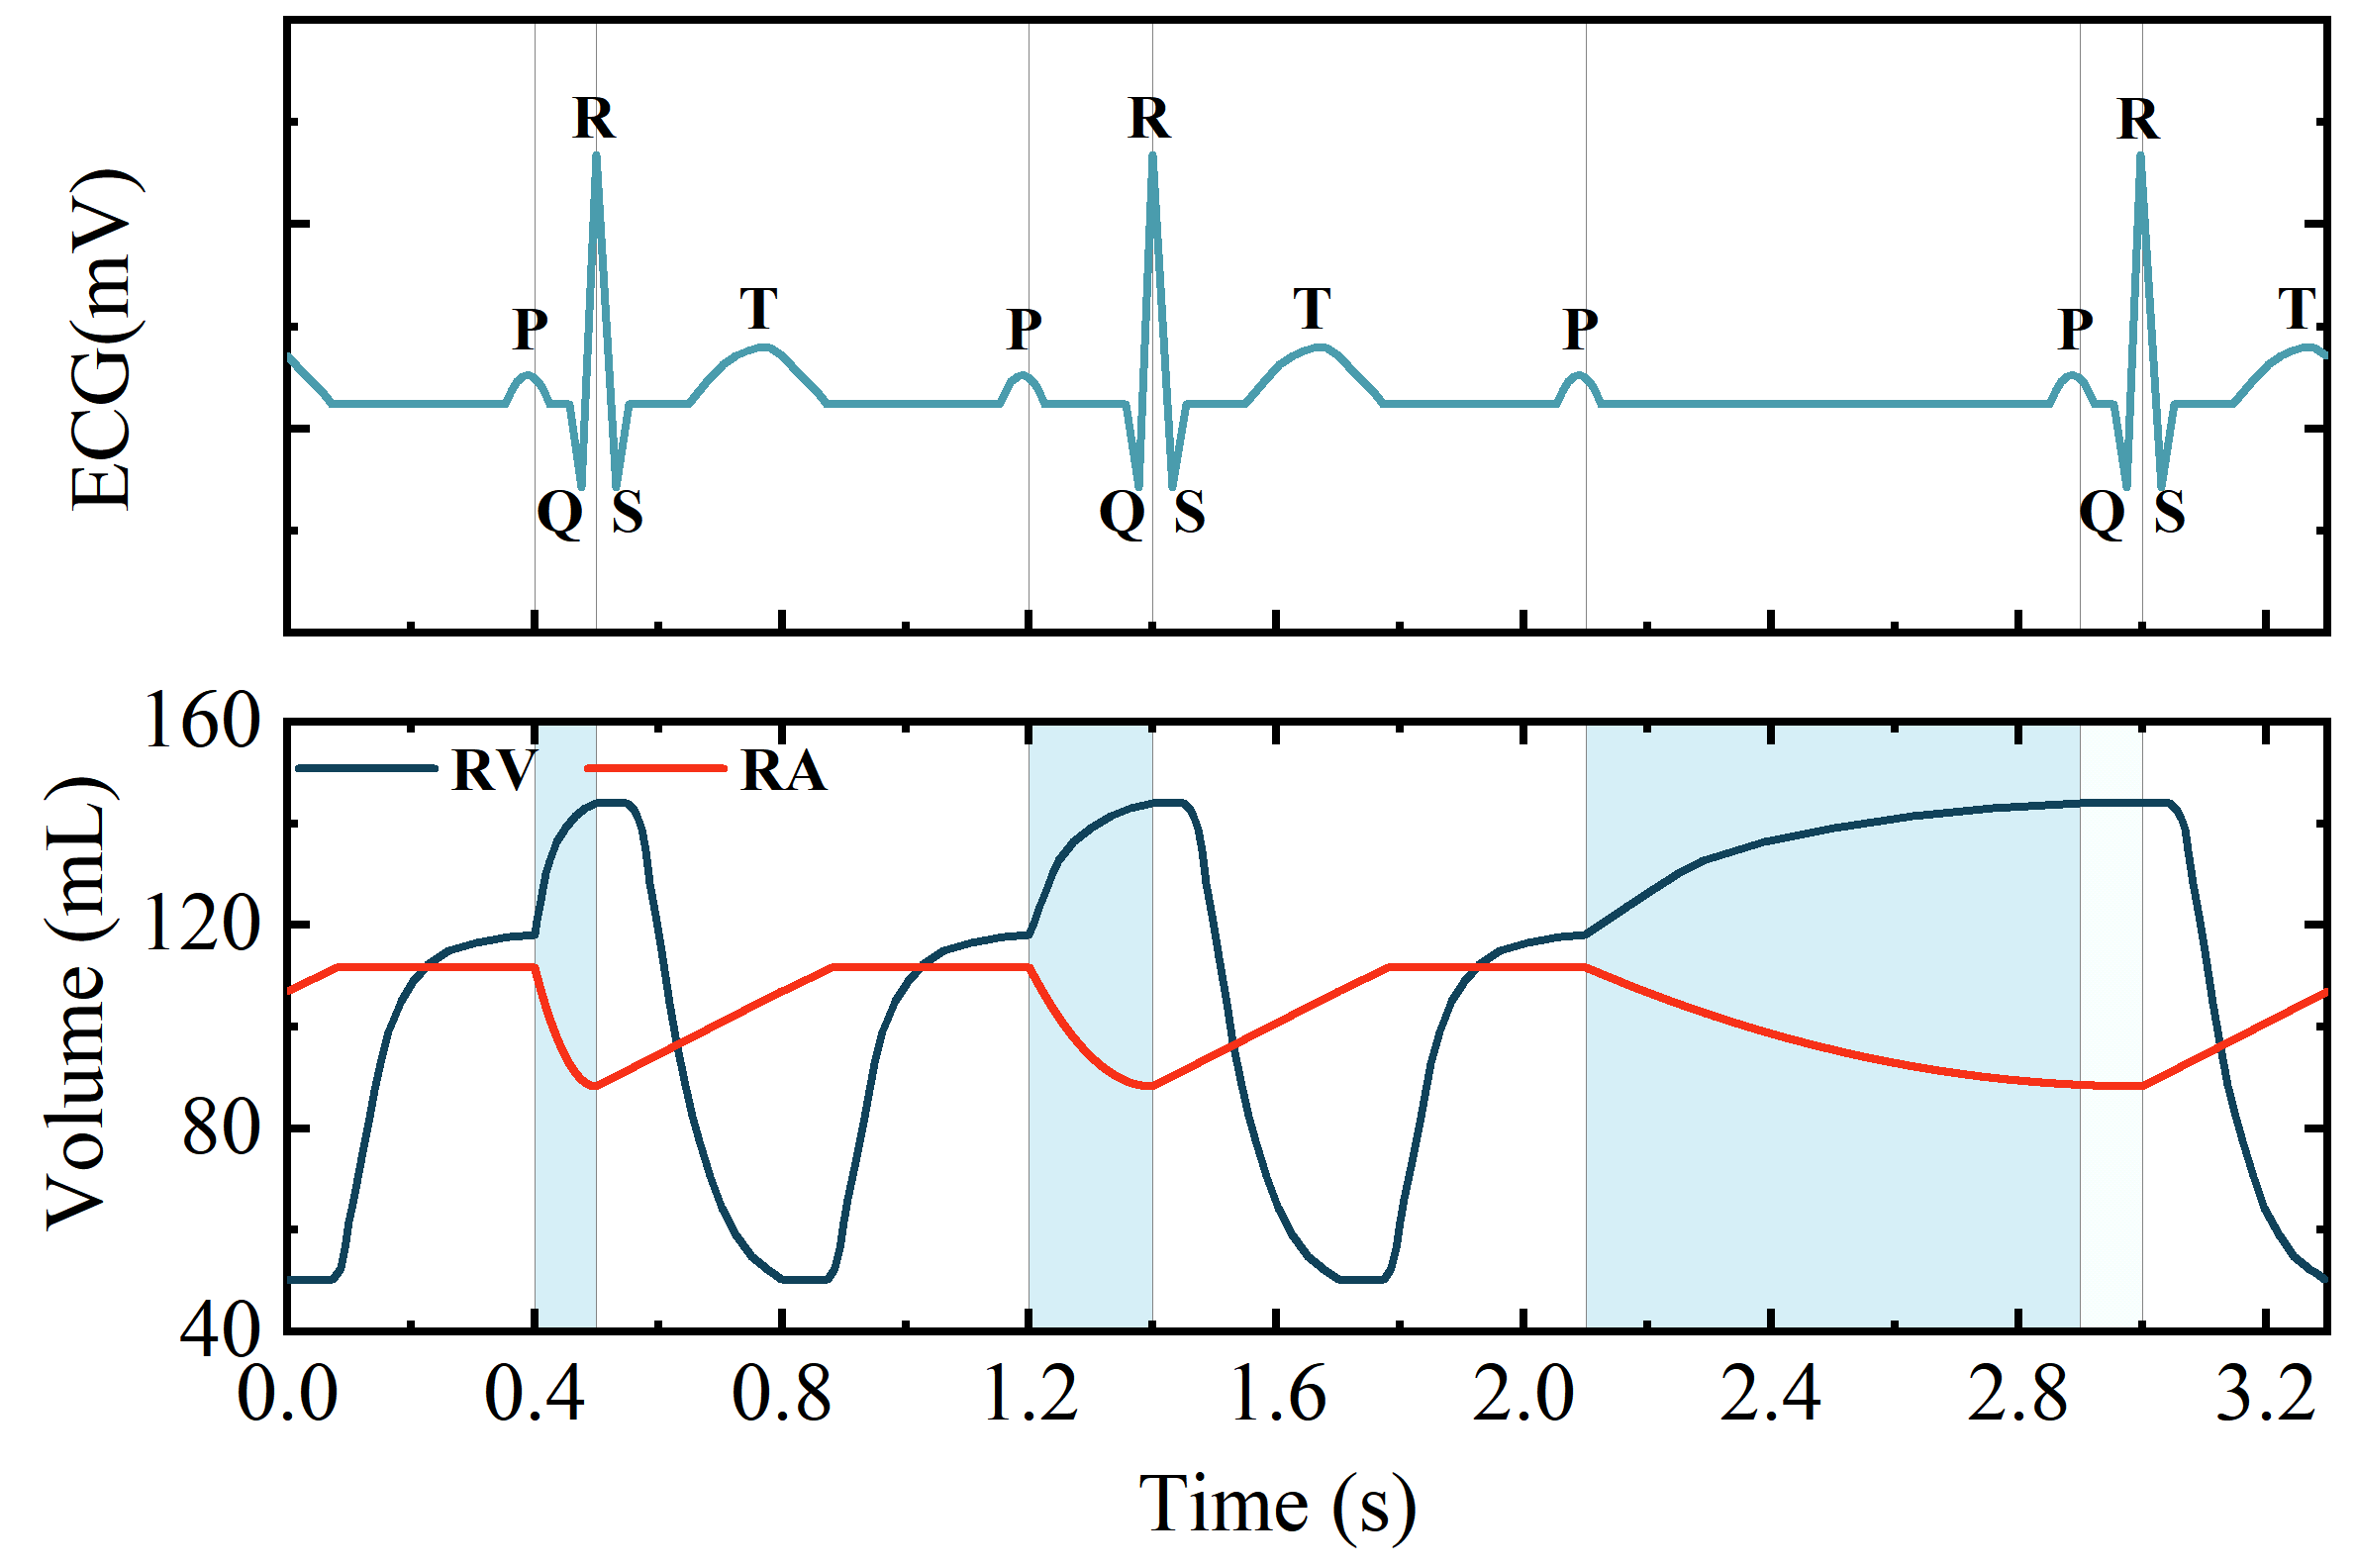
\includegraphics[width=0.9\columnwidth]{Figure/AVB_Vol} % 使用您的第三张图 (IMG_4224.jpeg)
    \caption{Emulation of a pathological cardiac cycle corresponding to an Atrioventricular Block (AVB) indication. The mapping illustrates an instance of intermittent conduction failure, where an atrial contraction (P-wave) is not followed by a ventricular response (QRS complex), leading to a distinct and irregular hemodynamic profile.}
    \label{fig:avb_mapping}
\end{figure}




\subsection{Communication System Evaluation Apparatus}




For the end-to-end performance evaluation of the communication system incorporating the AGC, the vector network analyzer was replaced by a complete transceiver link, with its block diagram depicted in Fig.~\ref{BER}.


The transmitter, comprising a signal generator, generated a 1-MHz carrier signal modulated with On-Off Keying (OOK). The amplitude of the sinusoidal carrier during the 'On' state was set to 100\,mV peak (V\textsubscript{p}) from the generator's 50\,\textOmega{} output, which corresponds to an average power of -10\,dBm. This modulated signal was then coupled into the cardiac tissue via an electrode implanted in the right atrium (RA).


Our custom-developed super-regenerative receiver (SRR), which integrates the proposed hybrid AGC circuit at its front-end, was connected to an electrode in the right ventricle (RV) for signal reception and demodulation.
All evaluations were conducted under the emulated atrioventricular block (AVB) conditions.



The experimental protocol began with an analysis of the system's dynamic behavior, where a digital storage oscilloscope was used to synchronously record the waveforms at critical nodes within the AGC loop and the end-to-end OOK demodulation process. Subsequently, the reliability of the communication link was quantitatively evaluated. The demodulated binary stream from the receiver was captured by a data acquisition (DAQ) system and compared offline against the known transmitted PRBS to calculate the Bit Error Rate (BER) over a data rate range of 500~bps to 5~kbps. Concurrently, the baseline BER performance without the AGC functionality was also evaluated. To ensure the reliability and repeatability of the results, all procedures were replicated across three independent porcine heart preparations (N=3). For each heart preparation, the BER measurement for each data point was repeated five times (n=5), and the results were averaged.


\begin{figure}[!t]
    \centering
    \includegraphics[width=0.95\columnwidth]{Figure/Mea.BER} % 使用您的第二张图 (实验装置图.png)
    \caption{Schematic diagram of the comprehensive experimental setup for the evaluation of the hybrid AGC super-regenerative receiver. The configuration integrates a signal generator (SG), an \textit{ex-vivo} porcine heart subjected to controlled perfusion to emulate dynamic intracardiac channel conditions, the super-regenerative receiver (SRR) incorporating the proposed AGC, and a data acquisition (DAQ) system. }
    \label{BER}
\end{figure}








\section{Experimental Results}
\label{sec:results}

The performance of the proposed hybrid analog-digital Automatic Gain Control (AGC) system for Super-Regenerative Receiver (SRR)-based intracardiac communication was rigorously evaluated.
The key findings are presented below, demonstrating the system's efficacy in mitigating dynamic channel variations, particularly under our simulated representative pathological condition.





\subsection{Dynamic Intracardiac Channel Characteristics}
Fig.~\ref{fig:path_gain_variation} illustrates the inherent dynamic variations in the Right Atrial to Right Ventricular (RA-RV) intracardiac channel path gain, measured over several cardiac cycles using an \textit{ex-vivo} porcine heart platform. Under simulated healthy heart conditions (Fig.~\ref{fig:path_gain_variation}(a)), the path gain exhibits periodic fluctuations of approximately \SI{10}{\decibel} to \SI{15}{\decibel}, synchronous with the cardiac mechanical activity. These variations become more pronounced and potentially irregular under simulated Mobitz Type I AVB conditions (Fig.~\ref{fig:path_gain_variation}(b)), with peak-to-peak fluctuations reaching up to \SI{15}{\decibel} to \SI{20}{\decibel}. Data from three different heart preparations (Heart-A, Heart-B, Heart-C) show consistent dynamic patterns, albeit with inter-subject variability. These results underscore the significant challenge posed by channel volatility to reliable Leadless Pacemaker (LCP) communication, necessitating an effective compensation mechanism.


%#图 \ref{fig:path_gain_variation} 展示了右心房到右心室（RA - RV）心内通道路径增益的固有动态变化，该变化是通过体外猪心脏平台在多个心动周期内测量得到的。在模拟的健康心脏条件下（图 \ref{fig:path_gain_variation}(a)），路径增益呈现出约10分贝到15分贝的周期性波动，与心脏机械活动同步。在模拟的莫氏Ⅰ型房室传导阻滞条件下（图 \ref{fig:path_gain_variation}(b)），这些变化变得更加明显且可能不规则，峰峰值波动可达15分贝到20分贝。来自三种不同心脏样本（心脏A、心脏B、心脏C）的数据显示出一致的动态模式，尽管存在个体间差异。这些结果凸显了通道波动性给可靠的无导线起搏器（LCP）通信带来的重大挑战，因此需要一种有效的补偿机制。

Fig.~\ref{fig:path_gain_variation} reveals the dynamic nature of the RA-RV intracardiac channel path gain. The results highlight a fundamental difference between ``healthy" and ``pathological" dynamics. Under simulated healthy conditions, as shown in Fig.~\ref{fig:path_gain_variation}(a), the path gain exhibits highly regular, periodic fluctuations that are strictly synchronized with the cardiac cycle. In stark contrast, under the simulated representative pathological conditions of Fig.~\ref{fig:path_gain_variation}(b), the nature of the channel dynamics changes radically. The most critical distinction is the loss of periodicity; due to the "dropped beats," the channel gain exhibits non-periodic, irregular behavior, making the timing and magnitude of its variations unpredictable. Data from three different heart preparations consistently reproduce this transition from ``regular" to``irregular," underscoring the profound challenge that such pathological dynamics pose to reliable LCP communication.



\begin{figure}[!t] % 使用 [H] 强制图片在当前位置 (需要 float 包)
    \centering
    % 假设您的图片文件名为 path_gain_variation.png/pdf/eps
    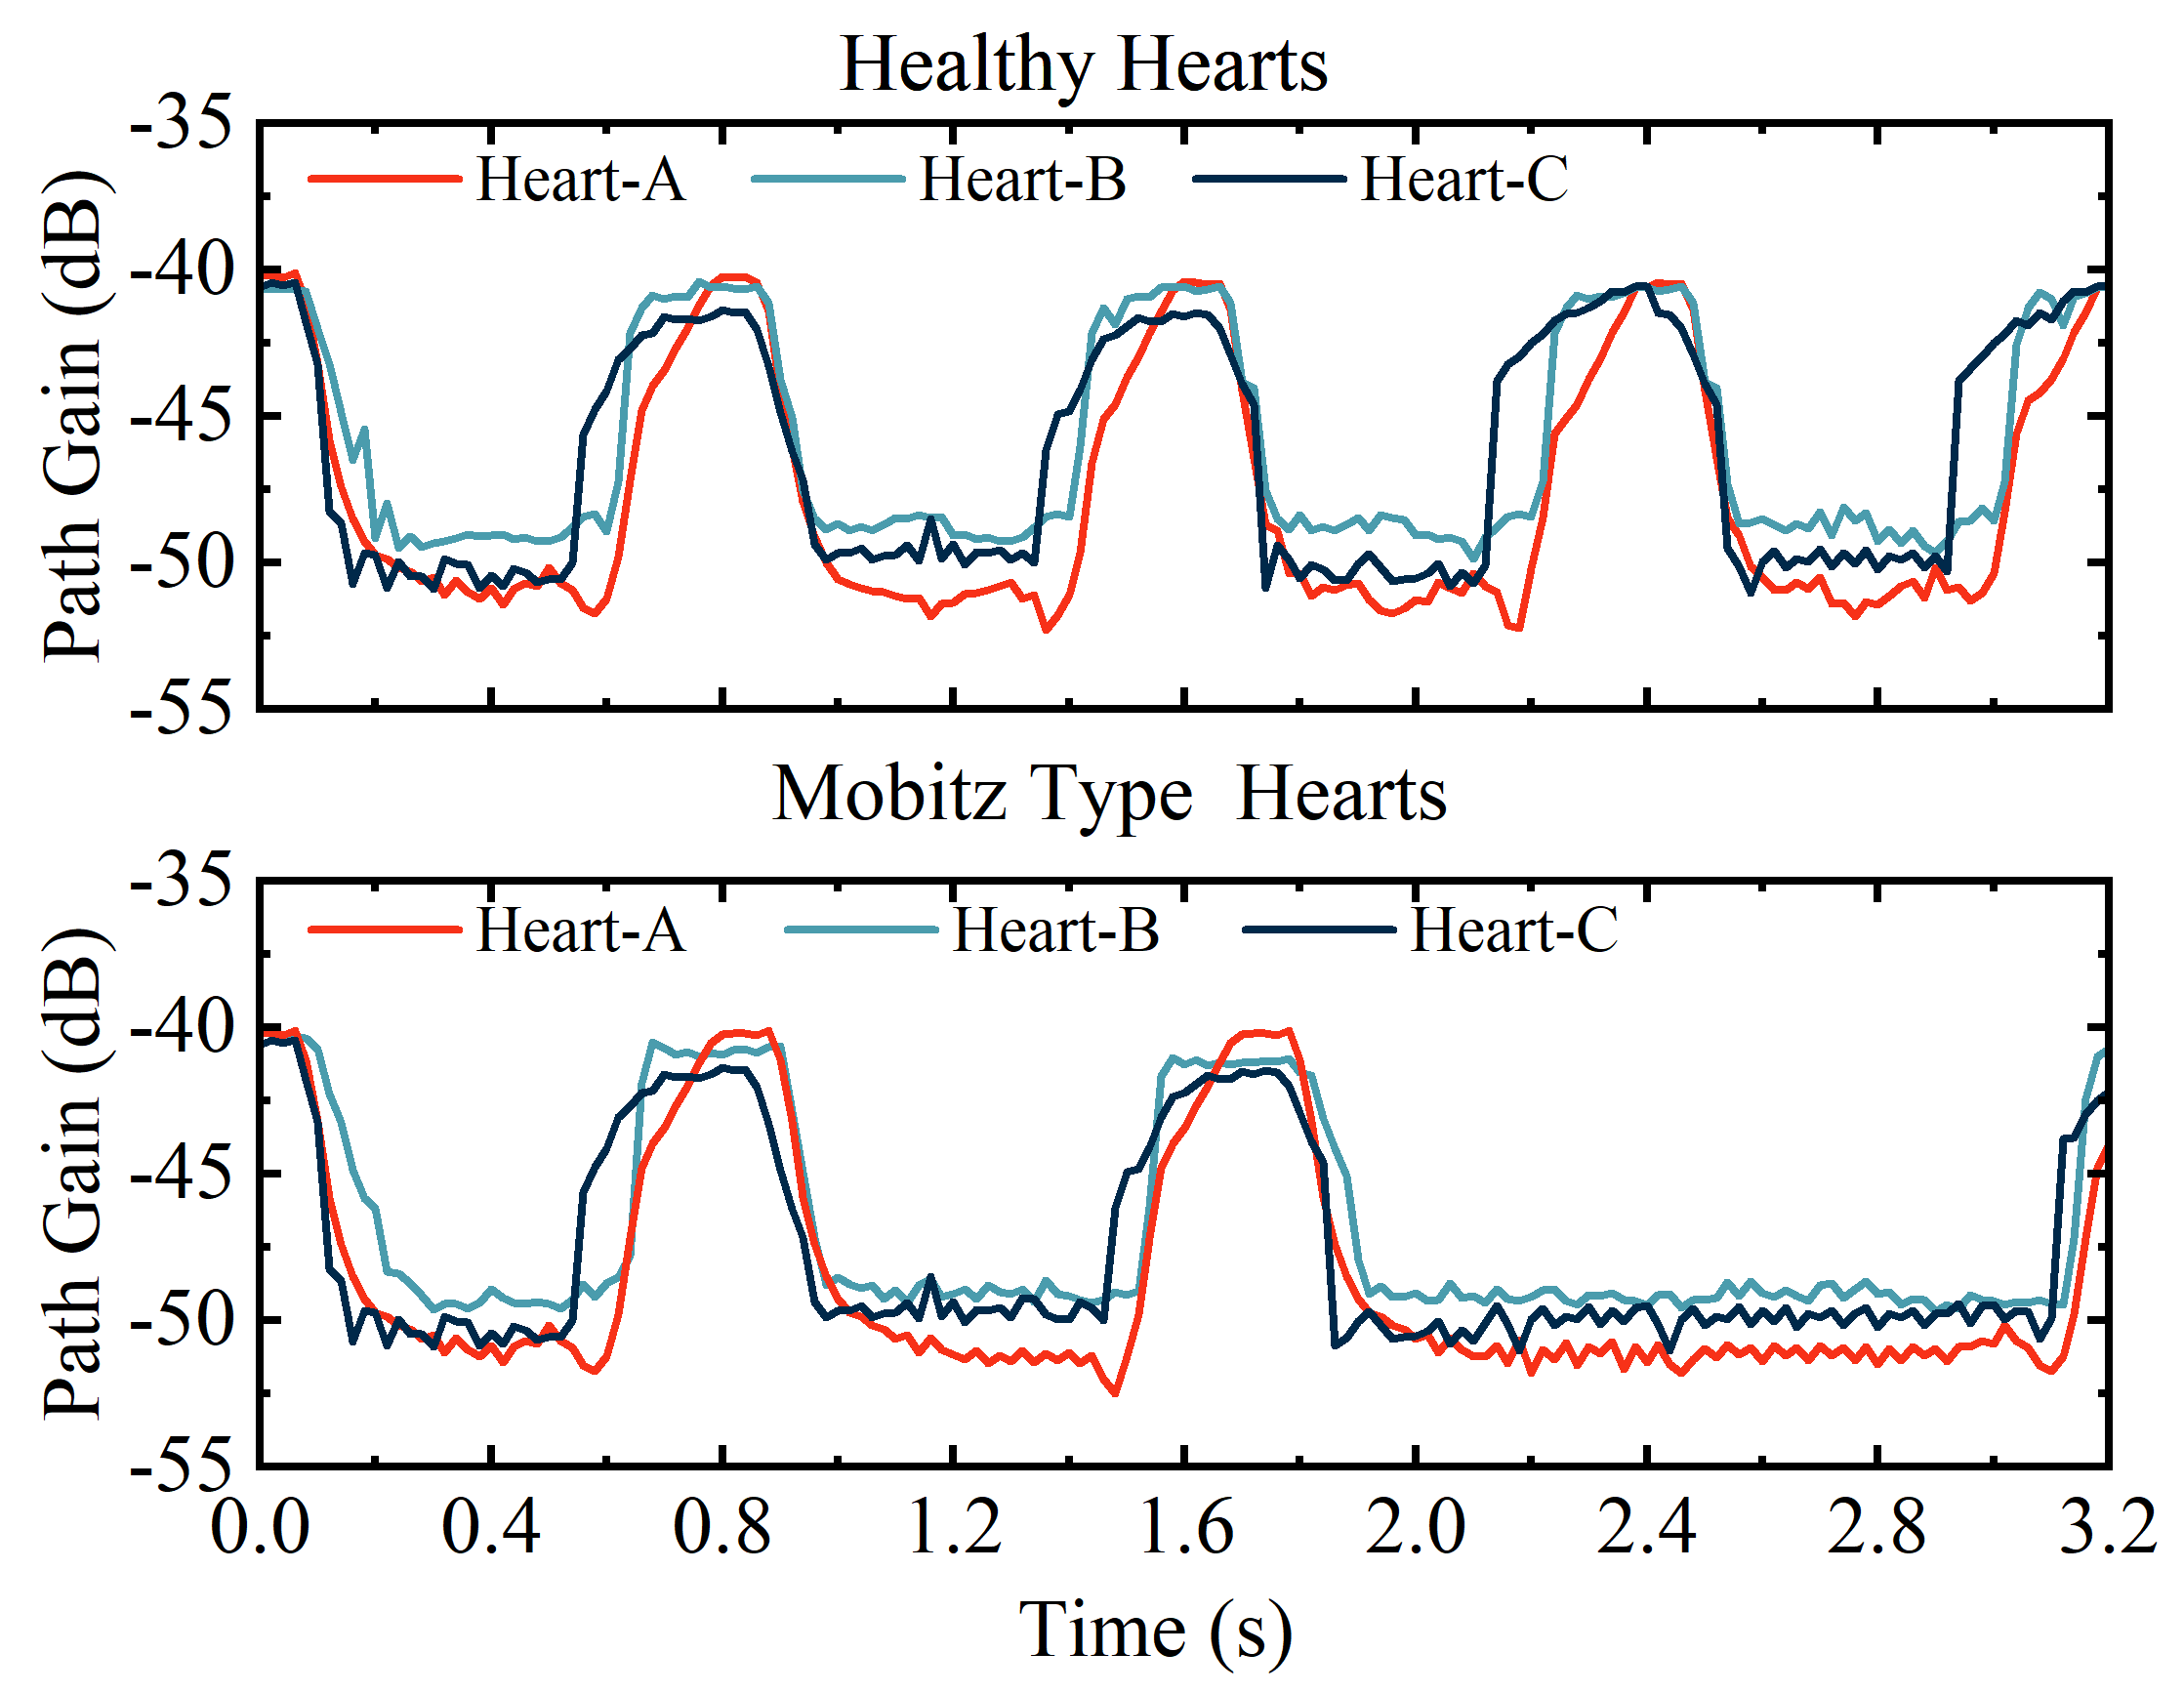
\includegraphics[width=0.9\linewidth]{Figure/signal_heart} % 替换为您的图片文件名
    \caption{Dynamic path gain variation of the RA-RV intracardiac channel. (a) Under simulated healthy heart conditions. (b) Under simulated representative pathological conditions. Results from three different ex-vivo porcine heart preparations (Heart-A, Heart-B, Heart-C) are shown.}
    \label{fig:path_gain_variation}
\end{figure}


\subsection{AGC System Performance in Signal Stabilization}
The effectiveness of the proposed hybrid AGC system in stabilizing the SRR input signal is demonstrated in Figure~\ref{fig:agc_stabilization}. The experiments were conducted under simulated Mobitz Type I AVB conditions, which induce severe channel dynamics. The reference Electrocardiogram (ECG) signal (Fig.~\ref{fig:agc_stabilization}(a)) provides a temporal marker for the cardiac cycle. Without AGC (Fig.~\ref{fig:agc_stabilization}(b)), the received signal amplitude at the SRR input (after the Low Noise Amplifier, LNA) fluctuated significantly from approximately \SI{1.5}{\milli\volt} to \SI{5.0}{\milli\volt}, directly reflecting the path gain variations observed in Fig.~\ref{fig:path_gain_variation}(b).

In contrast, when the hybrid AGC system was activated, the Proportional-Integral-Derivative (PID) controller dynamically adjusted the Variable Gain Amplifier (VGA) control voltage ($V_g$), as shown in Fig.~\ref{fig:agc_stabilization}(c). This control voltage, ranging from approximately \SI{12}{\milli\volt} to \SI{25}{\milli\volt}, exhibited an inverse relationship to the uncompensated signal amplitude, actively modulating the VGA gain to counteract channel losses or gains. Consequently, the SRR input signal amplitude was effectively stabilized around the target level of \SI{100}{\milli\volt} (Fig.~\ref{fig:agc_stabilization}(d)), with residual peak-to-peak fluctuations reduced to less than \SI{1}{\milli\volt} (i.e., approximately 1\%). This demonstrates the AGC's capability to provide a consistent signal level to the SRR despite substantial channel dynamics.



\begin{figure}[!t]
    \centering
    % 假设您的图片文件名为 agc_stabilization_effects.png/pdf/eps
    \includegraphics[width=0.9\linewidth]{Figure/Receiver_power} % 替换为您的图片文件名
    \caption{Effectiveness of the hybrid AGC system in stabilizing the receiver input signal under simulated Mobitz Type I AVB conditions. (a) Reference Electrocardiogram (ECG) signal. (b) Received signal amplitude at the SRR input without AGC. (c) Dynamic VGA control voltage ($V_g$) generated by the PID controller. (d) Received signal amplitude at the SRR input with the AGC activated, showing stabilization around the \SI{100}{\milli\volt} target.}
    \label{fig:agc_stabilization}
\end{figure}

\subsection{Impact of AGC on OOK Signal Demodulation}\label{subsec:impact-of-agc-on-ook-signal-demodulation}


Fig.~\ref{fig:ook_demodulation} provides compelling visual evidence of the proposed AGC's efficacy in enabling robust On-Off Keying (OOK) demodulation. The transmitted baseband sequence, with a logic-high level of 0.5\,V, is shown in Fig.~\ref{fig:ook_demodulation}(a). After passing through the adaptive front-end, the resulting signal at the SRR input is displayed in Fig.~\ref{fig:ook_demodulation}(b). Critically, even with the underlying dynamic channel, the AGC maintains the amplitude of the OOK bursts at a constant level, thereby presenting the SRR core with a stabilized signal ideal for demodulation.

Consequently, the SRR reliably recovers the data, producing the clean baseband output shown in Fig.~\ref{fig:ook_demodulation}(c). The output waveform's timing logic aligns perfectly with the transmitted sequence, and its high-level voltage of approximately 3.3\,V corresponds directly to the supply rail of the output comparator, confirming successful data recovery. This result qualitatively validates that the proposed AGC architecture is essential for preserving signal integrity and ensuring robust communication reliability amidst the challenging dynamics of the intracardiac channel.


\begin{figure}[!t]
    \centering
    % 假设您的图片文件名为 ook_waveforms.png/pdf/eps
    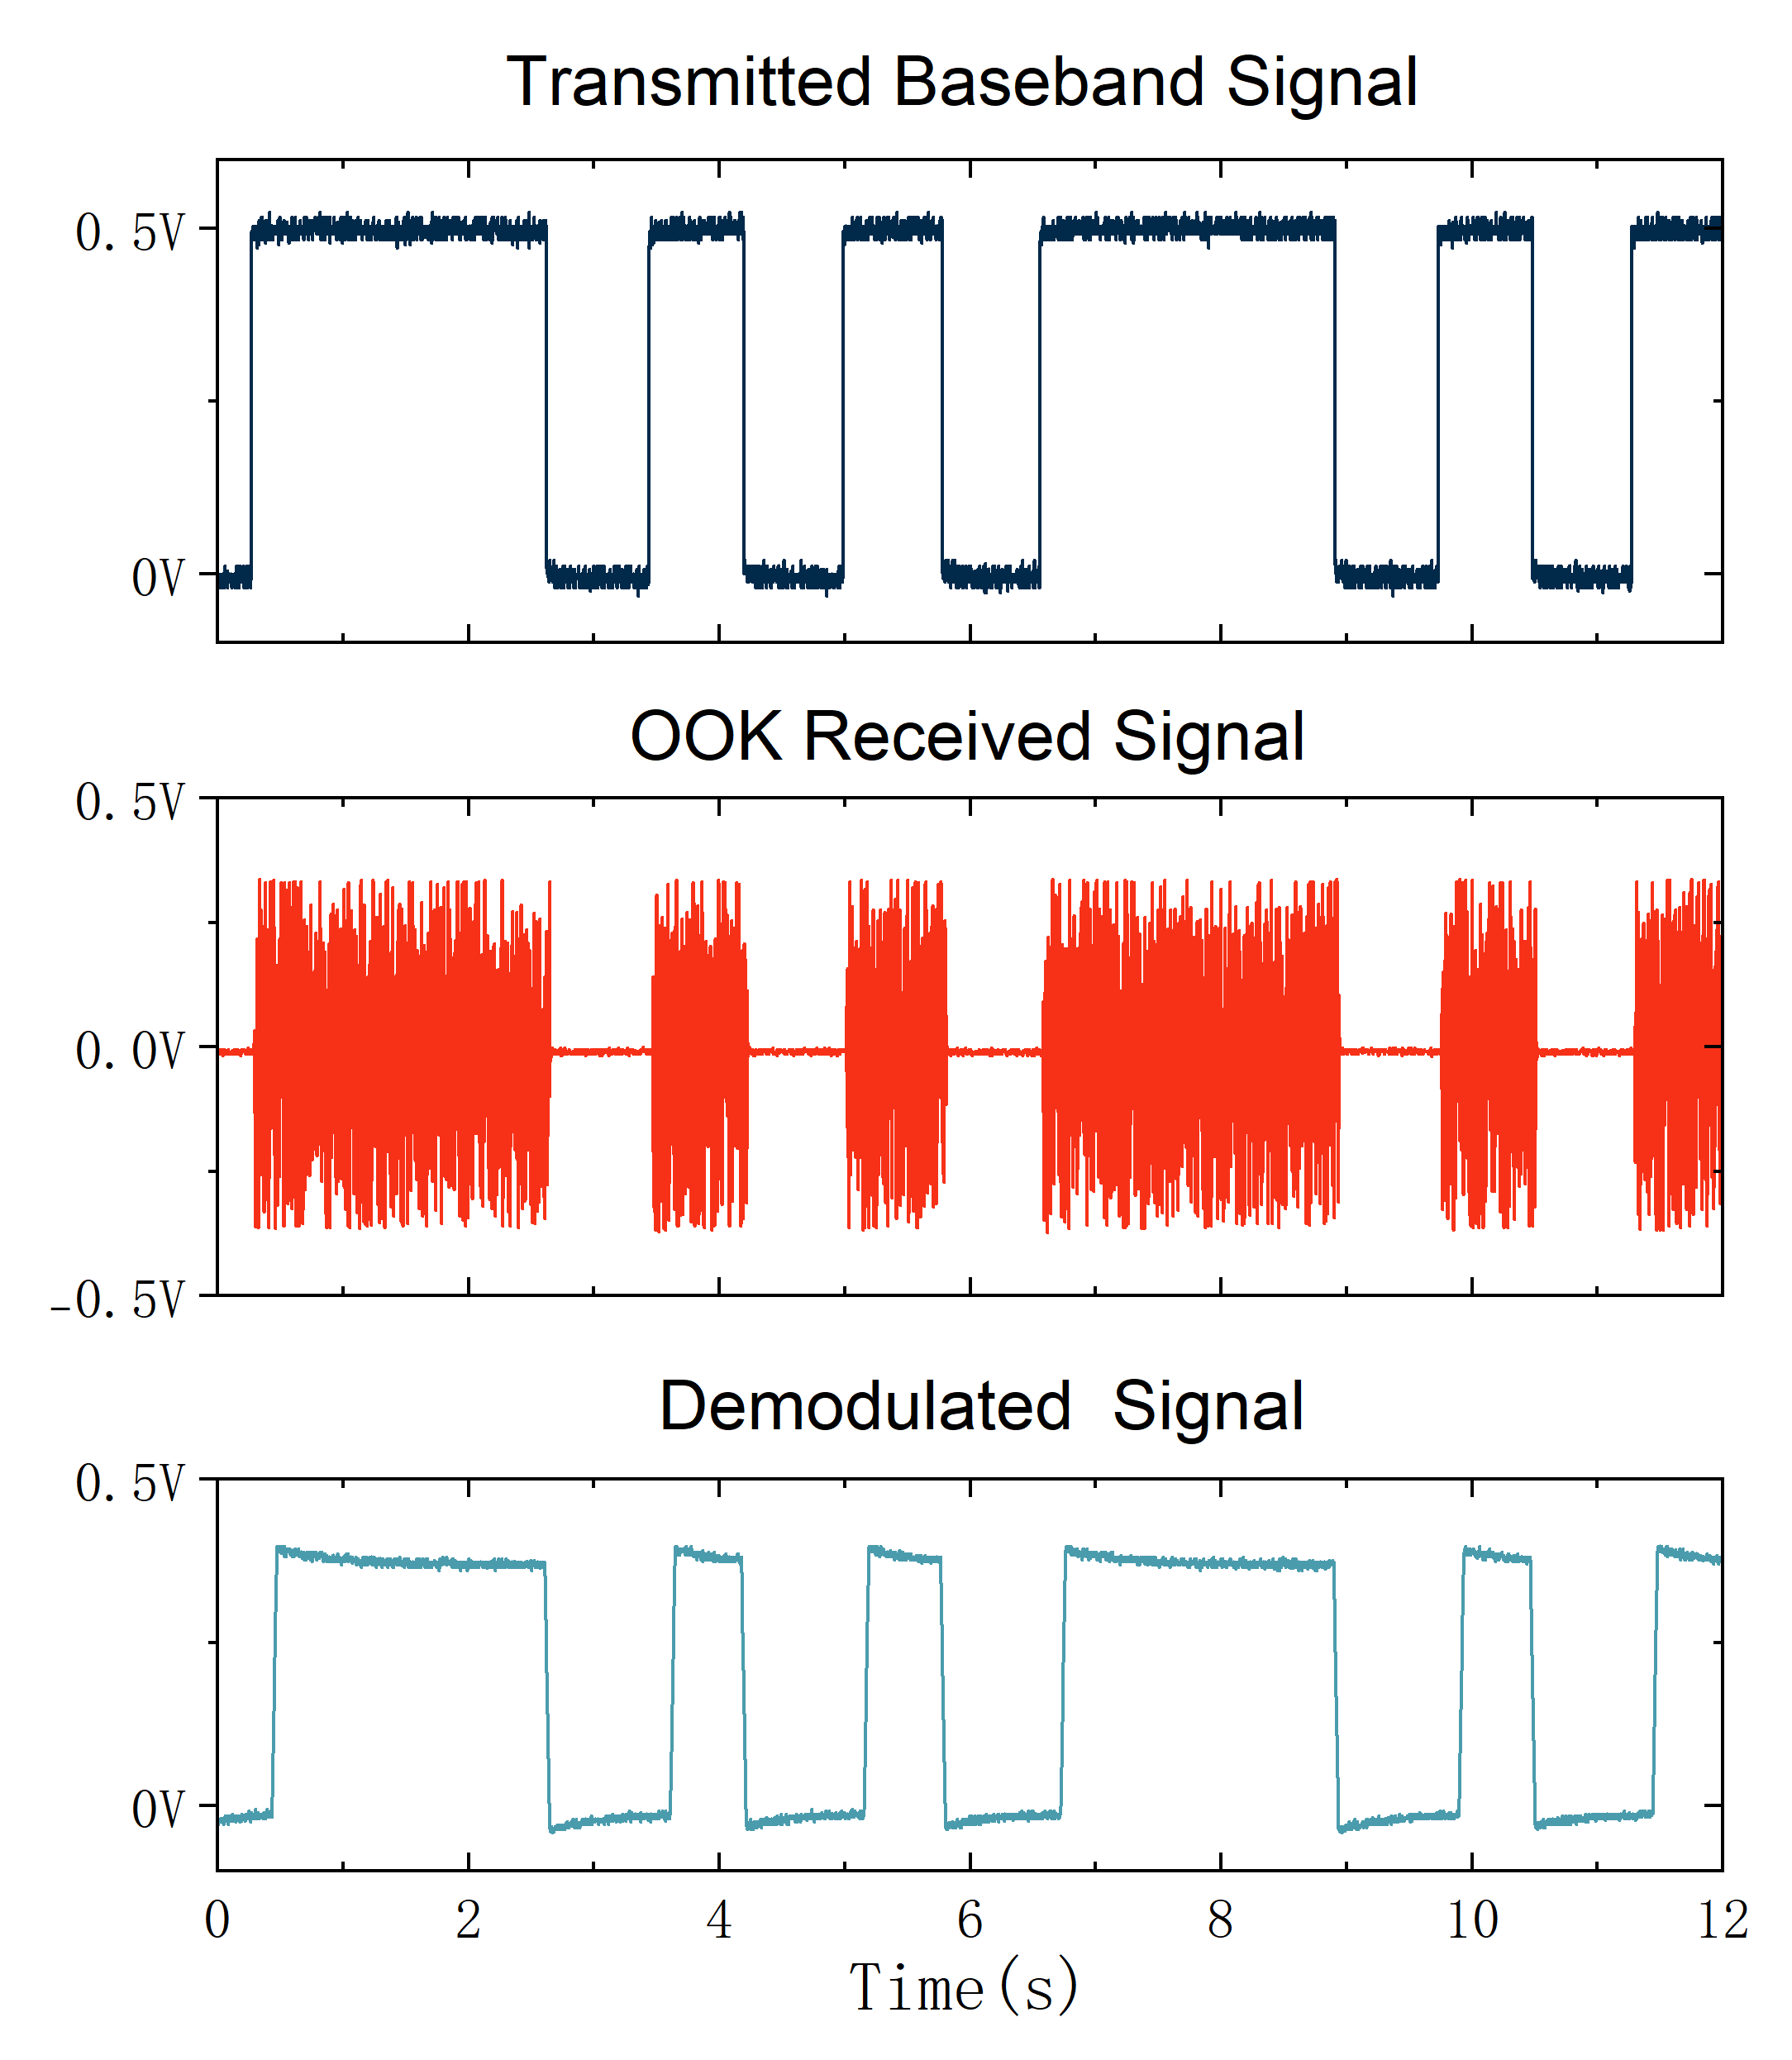
\includegraphics[width=0.8\linewidth]{Figure/ook} % 替换为您的图片文件名
    \caption{OOK signal waveforms at different stages of the communication system with AGC activated. (a) Transmitted baseband signal. (b) OOK received signal at the SRR input (after VGA with AGC). (c) Demodulated baseband signal at the SRR output.}
    \label{fig:ook_demodulation}
\end{figure}

\begin{figure}[!t]
    \centering
    % 假设您的图片文件名为 ber_vs_datarate.png/pdf/eps
    \includegraphics[width=0.8\linewidth]{Figure/BER} % 替换为您的图片文件名
    \caption{Bit Error Rate (BER) performance comparison with and without AGC across different data rates under simulated Mobitz Type I AVB conditions. The yellow line indicates the percentage improvement in BER achieved with AGC. Error bars represent the standard deviation across N=3 independent heart preparations, with each data point being the average of n=5 trials.}
    \label{fig:ber_performance}
\end{figure}

\subsection{Bit Error Rate (BER) Improvement}\label{subsec:bit-error-rate-(ber)-improvement}

%Quantitative assessment of the communication reliability was performed by measuring the Bit Error Rate (BER) with and without the AGC system across a range of data rates from \SI{500}{bps} to \SI{5}{kbps}, under simulated Mobitz Type I AVB channel conditions. As presented in Figure~\ref{fig:ber_performance}, the proposed AGC system significantly improved the BER performance. For instance, at a data rate of \SI{3}{kbps}, the BER was reduced from approximately \num{4.5e-4} (without AGC) to \num{9e-5} (with AGC). The percentage improvement in BER, calculated as (($\text{BER}_{\text{without\_AGC}} - \text{BER}_{\text{with\_AGC}}) / \text{BER}_{\text{without\_AGC}}) \times 100\%$, ranged from 54.8\% at \SI{500}{bps} to a substantial 83.7\% at \SI{5}{kbps}, as indicated by the yellow line and right y-axis.The small error bars in Fig.~\ref{fig:ber_performance}, representing the standard deviation across the three independent heart preparations (N=3), highlight the high consistency of these improvements and underscore the robustness of the proposed method across different biological samples.
%通过在模拟的莫比茨 I 型房室传导阻滞（AVB）信道条件下，测量有无自动增益控制（AGC）系统时，数据速率在500比特每秒（bps）至5千比特每秒（kbps）范围内的误码率（BER），对通信可靠性进行了定量评估。如图\(\ref{fig:ber_performance}\)所示，所提出的AGC系统显著改善了误码率性能。例如，在3 kbps的数据速率下，误码率从大约\(4.5\times10^{-4}\)（无AGC）降至\(9\times10^{-5}\)（有AGC）。误码率的改善百分比，按照\((\text{BER}_{\text{无AGC}} - \text{BER}_{\text{有AGC}}) / \text{BER}_{\text{无AGC}} \times 100\%\)计算，如黄色线条和右侧y轴所示，从500 bps时的54.8%到5 kbps时高达83.7%。图\(\ref{fig:ber_performance}\)中较小的误差棒代表三个独立心脏标本（\(N = 3\)）的标准差，突出了这些改善的高度一致性，并强调了所提出方法在不同生物样本中的稳健性。

To quantitatively evaluate the enhancement in communication reliability afforded by the AGC system, we systematically assessed the receiver's Bit Error Rate (BER) performance across various data rates under the challenging conditions of a simulated Mobitz Type I AVB channel.

The experimental results, presented in Fig.~\ref{fig:ber_performance}, provide indisputable evidence of the significant advantages of our proposed AGC system. Across the entire tested data rate range (\SI{500}{bps} to \SI{5}{kbps}), the BER with the AGC activated (blue bars) is consistently more than an order of magnitude lower than without it (red bars). For instance, at a data rate of \SI{3}{kbps}, the BER was reduced from approximately \num{4.5e-4} to \num{9e-5}, marking a qualitative leap for the communication link from a state of occasional errors to one of high reliability.

A more noteworthy trend is the systematic increase in the BER percentage improvement (indicated by the yellow line) with rising data rates, climbing from 54.8\% at \SI{500}{bps} to a substantial \textbf{83.7\%} at \SI{5}{kbps}. This phenomenon reveals a key insight: at higher data rates, the shorter duration of each symbol makes the system increasingly sensitive to any minor perturbation in signal amplitude. Therefore, the stable input provided by the AGC yields a greater "dividend" in maintaining demodulation performance at higher bitrates.

Finally, the small error bars in the figure, representing the standard deviation across N=3 independent heart preparations, provide strong statistical evidence for the robustness of our method. This indicates that the performance improvement brought by the AGC is not an artifact of a specific biological sample but is highly repeatable and generalizable across different subjects, a crucial factor for its practical clinical application.
%
%\begin{table*}[htbp]\caption{POWER PERFORMANCE COMPARISON WITH PREVIOUS CONDUCTIVE INTRABODY COMMUNICATION PROTOTYPES}
%    \label{table2}
%    \begin{threeparttable}
% \begin{tabularx}{\textwidth}{XXXXXX}
%\toprule
%
%\bfseries Publication   & \bfseries L. Bereuter et al.~\cite{bereuter2019leadless} &\bfseries  Ryser et al.~\cite{ryser2022modulation}& \bfseries Khaleghi et al.~\cite{khaleghi2020conductive} & \bfseries Yuk et al.~\cite{yuk2020implantable}  &\bfseries This work\tnote{a}
% \\
%\midrule
%\bfseries Measurement Type & In-vivo                   & In-vitro           & In-vitro       & In-vivo / In-vitro     & In-vitro  \\
%\bfseries Channel          & Porcine Heart             & Porcine Heart      & Porcine Heart  & Porcine Heart & Porcine Heart\\
%\bfseries Frequency [MHz]       & 1                        & 1.5               & 0.01-10       &DC-20  & 10   \\
%\bfseries TX Power[mW]\tnote{b}
%       & $>$360           & 97                 & 0.025     &0.57     & 198        \\
%\bfseries RX Power[mW]\tnote{b}
%     & $>$465            & 152   & 230   &0.062         & 390      \\
%\bfseries Technology       & Discrete                  & Discrete           & Discrete     &110nm CMOS  & Discrete      \\
%\bottomrule
%\end{tabularx}
%
% \begin{tablenotes}
%        \footnotesize
%        \item[a] The DDS is used for frequency adjustment, making it tunable.
%        \item[b] Only analog power.
%
%\end{tablenotes}
%
%\end{threeparttable}
%\end{table*}
\begin{table*}[htbp]
\centering
\caption{PERFORMANCE COMPARISON WITH RELATED RECEIVER PROTOTYPES}
\label{tab:comparison_modified}
% The 'threeparttable' environment is no longer needed since there are no footnotes.
% We use tabularx to make the table span the full text width and allow columns to wrap text automatically.
\begin{tabularx}{\textwidth}{l >{\raggedright\arraybackslash}X >{\raggedright\arraybackslash}X >{\raggedright\arraybackslash}X >{\raggedright\arraybackslash}X >{\raggedright\arraybackslash}X}
\toprule
\bfseries Metric & \bfseries Bereuter et al.~\cite{bereuter2019leadless} & \bfseries Rser et al.~\cite{ryser2022modulation} & \bfseries Khaleghi et al.~\cite{khaleghi2020conductive} & \bfseries Yuk et al.~\cite{yuk2020implantable} & \bfseries This Work \\
\midrule
\textbf{Core Contribution} & In-vivo Channel Characterization & Modulation Scheme Analysis & Wideband Channel Modeling & \textbf{Low-Power IC} & \textbf{Pathological Channel Robustness} \\
\addlinespace
\bfseries Measurement Type & In-vivo & In-vitro & In-vitro & In-vivo / In-vitro & \textbf{In-vitro (Simulated Pathology)} \\
\addlinespace
\bfseries Frequency [MHz] & 1 & 1.5 & 0.01-10 & DC-20 & 10 \\
\addlinespace
\bfseries RX Power [mW] & >465 & 152 & 230 & \textbf{0.062} & 268 \\
\addlinespace
\bfseries Technology & Discrete & Discrete & Discrete & \textbf{110nm CMOS} & \textbf{Discrete (Proof-of-Concept)} \\
\bottomrule
\end{tabularx}
\end{table*}


\section{Discussion}
\label{sec:discussion}

The experimental results of this study not only validate the effectiveness of our proposed hybrid AGC-SRR architecture but, more importantly, offer profound insights into understanding and countering the harsh intracardiac communication environment induced by pathological rhythms. Our core finding—a BER improvement of up to 83.7\% under simulated AVB conditions—transcends a mere numerical result. It experimentally quantifies for the first time the devastating impact of a "pathological channel" on communication reliability and eloquently demonstrates that active, real-time gain compensation is a fundamental strategy, not an optional optimization, for ensuring the reliability of LCPs in real-world clinical scenarios. The most critical insight from this work is the revelation that the design paradigm for communication systems must shift from adapting to the predictable, periodic fluctuations of a healthy heart to tracking the unpredictable, chaotic fluctuations of a pathological one.

The success of our proposed hybrid AGC architecture in tackling this challenge stems from its inherent design rationale. The effectiveness of the architecture can be intuitively understood from the waveforms in Fig.~\ref{fig:agc_stabilization}. The dynamic variation of the VGA control voltage ($V_g$) in Fig.~\ref{fig:agc_stabilization}(c) shows a clear inverse correlation with the uncompensated signal fluctuations in Fig.~\ref{fig:agc_stabilization}(b), indicating that the analog front-end can rapidly track channel transients caused by events such as dropped beats. Concurrently, the stabilized signal in Fig.~\ref{fig:agc_stabilization}(d), with its residual fluctuations suppressed to within 1\%, proves that the digital PID controller achieves high-precision steady-state control. It is precisely this combination of the analog front-end's rapid tracking capability and the digital back-end's precise steady-state control that enables the overall system to effectively combat aperiodic, severe fluctuations.

Placing this research within the evolutionary context of existing academic work highlights its pioneering nature. The early stages of intracardiac communication research, such as the work by Bereuter et al.~\cite{bereuter2019leadless_sync}, focused primarily on characterizing the channel's fundamental properties under static or quasi-static conditions, paving the way for the field. Subsequently, research entered a second phase, beginning to explore "healthy dynamics"; for instance, our team's prior work modeled the channel dynamics during a healthy cardiac cycle~\cite{wei2024time}. Together, these studies laid an essential foundation for understanding intracardiac communication. However, both static and healthy-dynamic models are confined to relatively idealized, predictable scenarios. The core contribution of this paper is to advance the research into a third, and most clinically challenging, stage: "pathological dynamics." We are the first to systematically shift the research focus to the irregular and unpredictable channel environment induced by a real-world pathology (exemplified by AVB) and to propose a validated adaptive receiver architecture designed to conquer such a harsh channel. This critical leap from "healthy" to "pathological" dynamics, along with the corresponding engineering implementation, represents a decisive step from foundational feasibility studies toward clinically robust applications.

We must also critically examine the boundaries and inherent limitations of this study. Our \textit{ex-vivo} porcine heart perfusion platform, while enabling the precise reproduction of hemodynamic and channel dynamics induced by our chosen representative pathology, cannot fully replicate all the complexities of a true in-vivo environment, such as real-time regulation by the autonomic nervous system and long-term tissue-electrode interface biological responses. Furthermore, our current system is a proof-of-concept prototype built from discrete, board-level components. Its value lies not in providing an immediately implantable device but in offering a rigorously validated, reliable design blueprint for future ASIC (Application-Specific Integrated Circuit) development at the system-architecture level. The use of discrete components provided the necessary flexibility for rapid iteration and validation of the core control algorithm.


Based on the foregoing analysis, the path for future research is clear. On the technological front, the primary task is the full-custom CMOS integrated circuit (ASIC) implementation of the validated hybrid AGC-SRR architecture, with the goal of reducing power consumption by at least an order of magnitude and achieving an implantable-grade miniature form factor. On the scientific front, it is necessary to advance our validation methodology from ex-vivo models to long-term in-vivo studies in large animal models, which will not only allow for the assessment of the system's long-term stability in a true in-vivo environment but also enable the investigation of a wider range of pathological models (such as more complex types of AV block or atrial fibrillation), ultimately propelling this promising technology toward clinical translation.

\section{Conclusion}
\label{sec:conclusion}

This paper confronted the core challenge of achieving robust communication for networked Implantable Medical Devices (IMDs) within dynamic, pathological biological environments. Using multi-chamber leadless pacemakers (LCPs) as a test case, we proposed and successfully validated a novel adaptive receiver architecture designed to conquer the severe and irregular channel fluctuations induced by pathological cardiac rhythms characterized by intermittent conduction failure.


Through rigorous testing on an \textit{ex-vivo} cardiac platform that we developed to precisely emulate a representative pathological dynamic, the architecture demonstrated exceptional performance. The results provide definitive proof that the proposed AGC system can stabilize the received signal to within 1\% of its target value amidst channel gain fluctuations exceeding \SI{15}{\decibel}, ultimately achieving a Bit Error Rate (BER) improvement of up to \textbf{83.7\%}.

In conclusion, this research not only provides a key enabling technology for clinically reliable multi-chamber LCPs but, more importantly, offers a rigorously validated and universally applicable design paradigm for the next generation of networked IMDs intended to operate robustly in harsh biological environments. Future work will focus on the CMOS integrated circuit implementation of this architecture to accelerate its translation to eventual clinical use.





\bibliographystyle{ieeetr}

\bibliography{Reference}

\end{document}


